\chapter{Patchy particle scheme for hydrophilic polymeric networks}

Now that we have covered the theoretical framework, we can delve into the numerical tools that will help us find relations between the polymeric network and the mechanical response.
First, we will describe the patchy particle scheme for simulating PNIPAM cross-linked networks.
Then, we will describe the numerical simulation protocol.
Next, we will introduce the LAMMPS package and explain how it can be used to simulate these systems.
Finally, we will present and analyze the simulation results.

\section{Simulation protocol}

One of the microgels that has been the focus of significant research is the type that is based on PNIPAM cross-linked networks.
In the article \textit{In silico Synthesis of Microgel Particles}\citep{gnanSilicoSynthesisMicrogel2017}, the authors present a flexible numerical protocol capable of designing individual microgel particles based on PNIPAM corr-linked networks. 
This protocol can generate particles with properties comparable to the experimental ones.
In this project, we employ a similar protocol to explore its versatility and identify a numerical tool that can facilitate connections between network configuration and mechanical response.

Our primary focus is on creating networks without spherical confinement and without mimicking the swelling behavior of PINIPAM microgels with temperature.
Therefore, the central strategy involves the implementation of a binary mixture of patchy particles to generate a disorded polymeric network structure, followed by the application of shear deformation.
The primary benefit of this protocol is that previous numerical efforts in microgel modeling have predominantly concentrated on unrealistic networks consisting of chains of equivalent length, frequently establishing cross-linked connections on crystalline lattice regions or where closed polymer networks are assembled by directly integrating randomly dispersed cross-linkers with polymer chains.

\subsection{Patchy particles representation}

A patchy particle\citep{bianchiPhaseDiagramPatchy2006,bianchiTheoreticalNumericalStudy2008} can be defined as a sphere with radius $r$ containing $n$ spheres of radius $l<r$ on its surface.
The smaller spheres are typically referred to as ``patches'' and the number of patches is often refer to as ``functionality''.
The center of the patches can be placed on the surface of the central particle. 
However, it can also be modified to be at a point inside the enclosed volume of the main particle.

The implementation of patchy particles as monomers and crosslinkers is a highly effective strategy.
This is due to the fact that it facilitates the integration of the infinitesimal representation by the Langevin dynamics with a particle that possesses volume and functionality.
The functionality representation is important because it allows for the representation of the monomer and cross-linker molecules that can form a polymeric network.
However, it is important to recognize that the geometry of the monomers and functional groups is assume to be spherical.

Finally, to define the volume of the particle, a repulsive pairwise interaction is defined between the central particles.
Meanwhile, to the formation of a polymeric network is facilitated by an attractive pairwise interaction defined between patches.
Because this model is designed to simulate the final network, not the synthesis process, the pairswise interaction between central particles and patches is not defined.

In contrast, the softness explain by particle interactions is characterized by the form of the repulsive pair potential between two particles.
Finally, the particle volume fraction contributes to the ability of the particles to deform or compress, in contrast to hard spheres\footnote{The patchy particles are hard spheres, but the hydrogel network is a soft ``particle''}\citep{vlassopoulosTunableRheologyDense2014}.

\subsection{Description of the system}

%\paragraph{Interaction potentials} 
We start by describing the interaction potentials between patchy particles.
The interaction between the central particles is modeled with a Weeks-Chandler-Andersen repulsive potential,
\begin{gather}
    U_{WCA}(r_{i,j}) =\left\{ 
        \begin{array}{ll}
            4\epsilon_{i,j}\left[\qty(\frac{\sigma}{r_{i,j}})^{12}-\qty(\frac{\sigma}{r_{i,j}})^6\right]+\epsilon_{i,j}, & r_{i,j}\in[0,2^{1/6}\sigma], \\
            0, & r_{i,j}>2^{1/6}\sigma
        \end{array}
\right.
    ,\label{eqn:CL-MO_interaction}
\end{gather}
where $r_{i,j}$ is the distance between the center of the central particles, $\sigma$ is the diameter of the particles and $\epsilon_{i,j}$ is the energy of the interacton.
On the other hand, the patch-patch interaction is modeled with an attractive potential,
\begin{gather}
    U_{\mathrm{patchy}}\qty(r_{\mu\upsilon}) = \left\{
        \begin{array}{ll}
            2\epsilon_{\mu\upsilon}\left(\frac{\sigma_p^4}{2 r_{\mu\upsilon}^4}-1\right)\exp\left[\frac{\sigma_p}{\qty(r_{\mu\upsilon}-r_{c})}+2\right], & r_{\mu\upsilon}\in\qty[0,r_c], \\
            0, & r_{\mu,\upsilon}>r_c,
        \end{array}
            \right.\label{eqn:patch-patch_interaction}
\end{gather}
where $r_{\mu\upsilon}$ is the distance between two patches, $\sigma_p$ is the diameter of the patches, $r_c$ is the cut distance of interaction set to $1.5\sigma_p$ and $\epsilon_{\mu,\upsilon}$ is the interaction energy between the patches.
%This potential can be interpreted as a reversible interaction.

In figure~\ref{fig:patchpatchpot} is a contrast between the patch-patch interaction potential~\eqref{eqn:patch-patch_interaction}, the Lennard-Jones potential and the FENE potential.
Qualitatively, the Lennard-Jones and the patch-patch potential are similar, in the sense that after a cut off distance, both potentials tends to zero.
In contrast, the FENE potential goes to infinity if the distance is to short or to wide.
This main difference allow us to implement the patch-patch interaction as a reversible interaction, rather than the FENE, which is more suitable to represent non-reversible interaction.
Hence, this numerical methodology is like having a polymeric network with physical crosslinkers.

\begin{figure}[ht!]
    \centering
    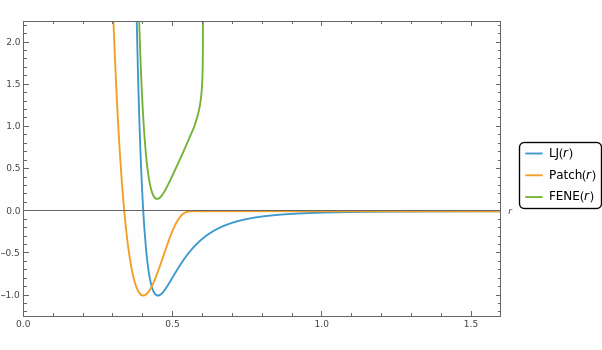
\includegraphics[width=0.8\textwidth]{figs/numerical/patchpatch.png}
    \caption{Comparisson between equation~\eqref{eqn:patch-patch_interaction} with Lennard-Jones and FENE potentials.}\label{fig:patchpatchpot}
\end{figure}

In contrast, the difference between the Lennard-Jones potential with patch-patch interaction is that the minimum potential undergoes horizontal translation, and the rate of change from the minimum to the cut distance is more pronounced in the patch-patch interaction.
This translates into a more ``strong'' interaction between the patches using equation~\eqref{eqn:patch-patch_interaction} than a Lennard-Jones potential.

In addition, if we let the polymeric network form with the interaction of equation~\eqref{eqn:patch-patch_interaction}, the patches are going to form cluster of more than 2 patches, which is not desirable.
Hence, the interaction between patches is complemented by a three-body repulsive potential, defined in terms of~\eqref{eqn:patch-patch_interaction}, that provides an efficient bond-swapping mechanism making possible to easily equilibrate the system at extremely low temperatures, while at the same time, reataining the single bond per patch condition\citep{sciortinoThreebodyPotentialSimulating2017},
\begin{gather}
    U_{\mathrm{swap}}(r_{l,m},r_{l,n}) = w\sum_{l,m,n}\epsilon_{m,n}U_3\qty(r_{l,m})U_3\qty(r_{l,n}),\quad r_{l,n}\in\qty[0,r_c],\label{eqn:swap_interaction}
\end{gather}
where
\begin{gather}
    U_{3}\qty(r) = \left\{
        \begin{array}{ll}
            1 & r\in\qty[0,r_{\min}], \\
            -U_{\mathrm{patchy}}\qty(r)/\epsilon_{m,n}, & r\in\qty[r_{\min},r_c]
        \end{array}
        \right.\label{eqn:swapmod_interaction}.
\end{gather}
The sum in~\eqref{eqn:swap_interaction} runs over all triples of bonded patches (patch $l$ bonded both with $m$ and $n$).
$r_{l,m}$ and $r_{l,n}$ are the distances between the reference patch and the other two patches.
The parameter $\epsilon_{m,n}$ is the energy of repulsion and $w$ is used to tuned the swapping ($w=1$) and non-swapping bonds ($w\gg1$). 
The cut off distance $r_c$ is the same as in the potential of interaction between patches, meanwhile the minimum distance $r_{\min}$ is the distance at the minimum of~\eqref{eqn:patch-patch_interaction}, \textit{i.e.} $\epsilon_{m,n}\equiv\abs{U_{\mathrm{patchy}}(r_{\min})}$.

In figure~\ref{fig:swappot} shows the patch-patch potential with the swap potential.
The patch-patch potential in the figure is the energy of the interaction between patch $i$ with patch $k$.
The swap potential is the energy between patch $i$ with patch $k$ leaving the distance between patch $i$ and patch $j$ fixed.
Tacking into account this, when the patches $i-j$ are at the potential well ($r_{ij}=\sigma$), the interaction between $i-k$ is null.
When the patches $i-j$ is bigger than the potential well but smaller than the cutoff distance ($r_{\mathrm{cut}}>r_{ij}>\sigma$), the interaction between $i-k$ is mild attractive.
Finally, when the patches $i-j$ is bigger than the cutoff distance ($r_{\mathrm{cut}}<r_{ij}$), the interaction between $i-k$ is attractive.

\begin{figure}[ht!]
    \centering
    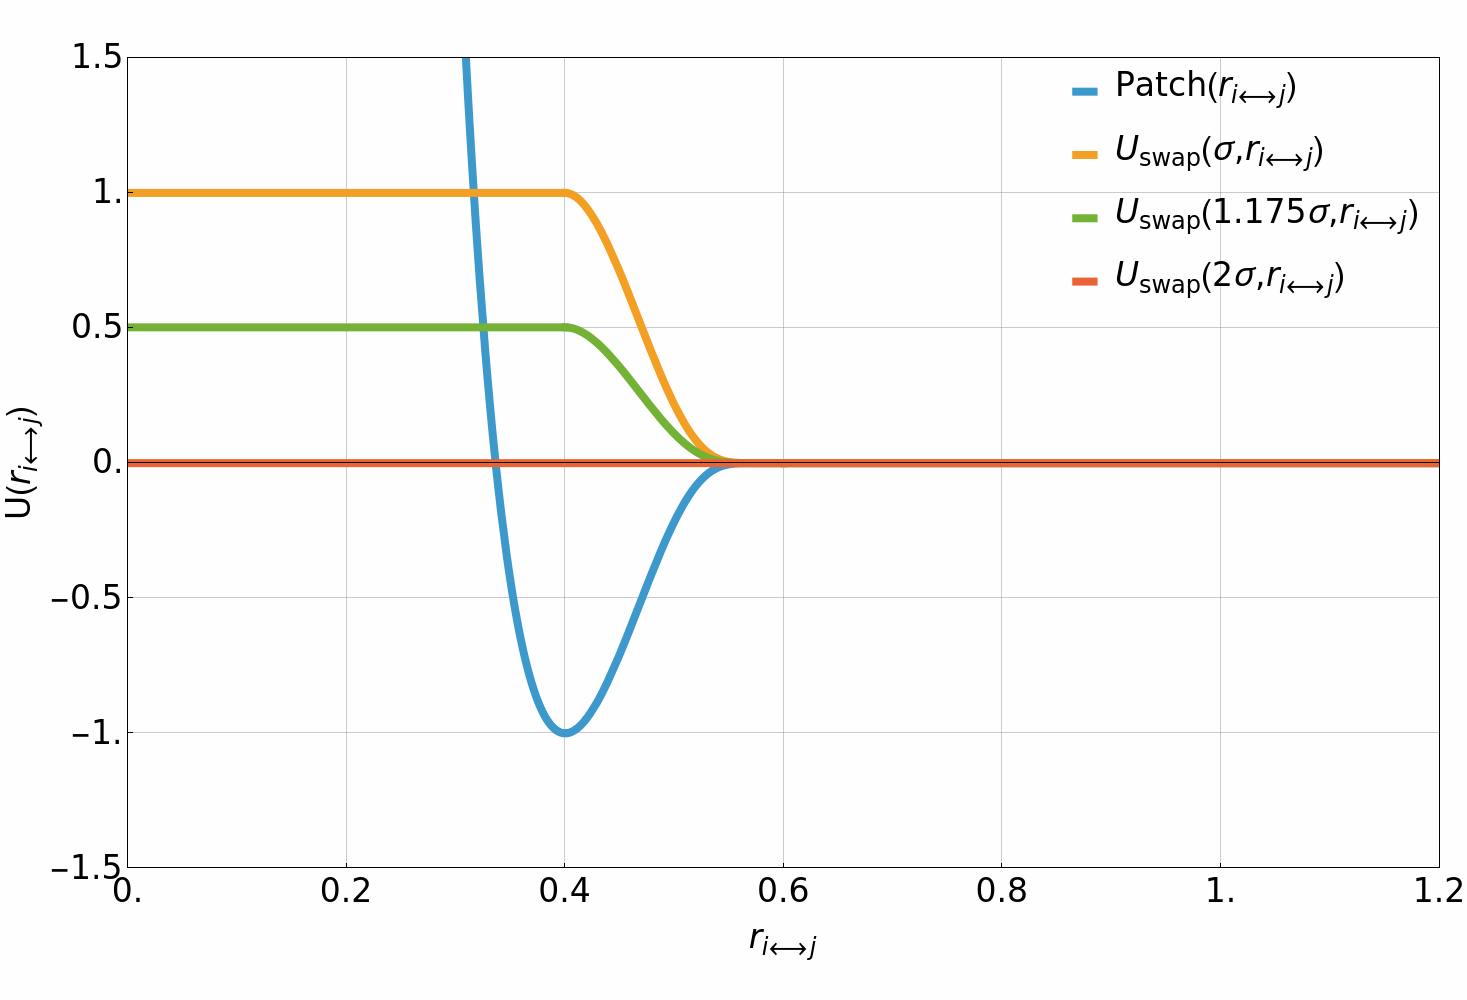
\includegraphics[width=0.8\textwidth]{figs/numerical/swapPotential.png}
    \caption{Swap potential for patch-patch interaction to ensure single bond per patch condition.}\label{fig:swappot}
\end{figure}

Before proceeding to the description of the parameteros for the simulation, it is necessary to describe the interaction between the central particle and the patches.
The patches and the central particles are linked by harmonic potentials,
\begin{align}
    E_r &= K_r\qty(r-r_{o})^2, \\
    E_\theta &= K_\theta\qty(\theta-\theta_{o})^2.
\end{align}
Where $r_o$ and $\theta_o$ represent the equilibrium bond distance and angle.
Meanwhile, $K$ is equal to $K=k/2$, where $k$ is the energy of the bond.
This allow us to create patchy particles with patches fixed at a convinient position.

%\paragraph{Polymeric network parameters}
Now that the interaction between pathcy particles have been described, we can describe the control parameters for the simulations.
We set a constant number of patchy particles $N_p$, a packing fraction $\phi$ and a cross-link concentration $c$. 
From this parameters we compute the volume of the box and the number of patchy particles of functionality 2 (PB) and the patchy particles of functionality 4 (PA).

Due to limitations related to time and computing resources, we have set the total number of particles to be $N_p=\num{8000}$.
This is a lower number of particles when compared with other simulations[cites].
Therefore, in order to compensate, we take the mean of five experiments.
In addition, the timestep was set to \num{0.001}, as a good rule of thumb\footnote{Talk about LJ units.}.
This is equivalent to simulating a system of \num{40000} particles, but with a more manageable computational requirements.
Finally, the values of $K_r$ and $K_\theta$ is set to \num{100}, to create a strong bond and prevent stretching.
The value of $r_o$ is set to \num{0.45}.
The value of $\theta_o$ is set to \SI{180}{\degree} for PB particles and \SI{109.4712}{\degree} for PA particles.

Once we set the parameters for the synthesis, the volume of the box was calculated by determining the volume of the patchy particles A and B, and then scaling those values by the number of particles and the desired packing fraction.
\begin{align*}
    V_{\mathrm{box}} &= \frac{N_{\mathrm{patchyA}}V_{\mathrm{patchyA}}+N_{\mathrm{patchyB}}V_{\mathrm{patchyB}}}{\phi}
\end{align*}
The number of patchy particle of type A is computed as $N_{\mathrm{patchyA}} = c N_p$ and the number of patchy particles of type B as $N_{\mathrm{patchyB}}= N_p - N_{\mathrm{patchyA}}= N_p(1 - c )$.
Finally, the temperature was set to be constant thru all the assembly process $T=\num{0.05}$ in Lennard-Jones units, meanwhile, the damp parameter was set to $\mathrm{damp}=\num{0.5}$.
It is important to notice that the damp controlls the viscous response from the interaction between the thermal bath and the particles, which represents the interaction between water molecules and the polymer network.

We set the radius of the central particle at $0.5$ ($\sigma=1$) and the radius of the patches at $0.2$ ($\sigma_p=0.4$).
The energy of interaction between central particles is 1 $\epsilon_{i,j}=1$.
In constrast, the energy of interaction between patches is difend as follows,
the interaction between patches of patchy particles with two patches is set to 1 ($\epsilon_{\mu,\upsilon}=1$), 
the interaction between patches of patchy particles with four patches is set to \num{0} ($\epsilon_{\mu,\upsilon}=0$) 
and the interaction between patches of patchy particles with four patches with patchs of patchy particles of two patches is set to \num{1} ($\epsilon_{\mu,\upsilon}=1$).
This is to allow only crosslinker-monomer and monomer-monomer bonding.

%\paragraph{Deformation protocol}
Once the assembly simulation of the patchy particles network was done, we peform a shear deformation to the resulting network.
We select the shear deformation because shear forces dominate biological environments where hydrogels are typically deployed. 
Also, shear testing provides a more uniform stress field throughout the hydrogel sample compared to tensile testing. 
In rheological measurements using parallel plate or cone-and-plate geometries, the applied shear stress is distributed evenly across the sample, eliminating edge effects and stress concentrations that plague tensile testing.
Furthermore, shear rheometry excels at characterizing the complex viscoelastic properties that define hydrogel functionality.
Many hydrogels exhibit shear-thinning behavior that is critical for applications like injection and 3D bioprinting. 

The shear deformation was done at a constant shear rate in the $xy$ plane.
The shear rates where in the \num{d-3} order of magnitude and final strain was \num{15} units.
This is because we are exploring this computational methodology to characterized the mechanical response and to deform beyond the plastic deformation limit.
Also the variation of the shear rate was perform to see the viscoelastic response of the material.
The temperature and damp parameter where set to be the same as in the assembly process.

\subsection{LAMMPS implementation}

As said before, we take advantage of the LAMMPS software as a computational tool to solve the langevin equation in a many-particle system.
However, it is usefull to explain how we apply the simulation in this software.
In this regard, we discuss briefly the $\mathrm{damp}$ parameter, the implementation of the swap potential~\eqref{eqn:swapmod_interaction}, the shear deformation and the calculation of the stress tensor.

%\paragraph{damp}
As we saw in equations~\eqref{eqn:MolDylammps1} and~\eqref{eqn:MolDylammps2}, the viscosity parameter $\gamma$ of the lagevin equation~\eqref{eqn:BrownianDyn1} does appears, instead the $\mathrm{damp}$ parameter appears.
This parameter is specified in time units and determines how rapidly the temperature is relaxed so that can be more easily be used as a thermostat\citep{LAMMPS}.
That is, if damp is set to \num{100}, the temperature will relax in a timespan of roughly \num{100} time units.
By making dimensional analysis, the damp factor can be think as inversely related to the viscotity of the solvent.
This tells us that a small damp represents a high-viscosity solvent and vice versa.
Therefore, since we set this parameter to \num{0.1} the polymeric network is in a high-viscosity solvent.

%\paragraph{Three-body potential}
Now moving towards the implementation of the swap-potential.
We use the \verb|pair_style threebody/table| command because it allow us to implement a generic tabulated three-body interactions.
However, in lammps, the tabulation is done on a three-dimensional grid of the two distances $r_{ij}$ and $r_{ik}$ as well as the angle $\theta_{ijk}$, where the forces on all three particles $I$, $J$, and $K$ lie within the plane defined by the three inter-particle distance vectors $\vec{r}_{IJ}$, $\vec{r}_{IK}$ and $\vec{r}_{JK}$\citep{LAMMPS}.
Allowing the following property to project the forces onto the inter-particle distance vectors,
\begin{equation}
    \begin{pmatrix}\vec{f}_i \\ \vec{f}_j \\ \vec{f}_k\end{pmatrix}
    =
    \begin{pmatrix}f_{i1} & f_{i2} & 0 \\ f_{j1} & 0 & f_{j2} \\ 0 & f_{k1} & f_{k2} \end{pmatrix}
    \begin{pmatrix}\vec{r}_{ij} \\ \vec{r}_{ik} \\ \vec{r}_{jk}\end{pmatrix}.
\end{equation}
And due to symmetry reasons, we have that $f_{i1}=-f_{j1}$, $f_{i2}=-f_{k1}$ and $f_{j2}=-f_{k2}$.
Hence, we need to project the force of the swap potential into the inter-particle plane in order to have a correct tabulation.

Recalling that the force is equivalent to $-\nabla U(r)$ and the potencials has only radial dependence, we can express the force as,
\begin{gather}
    \vec{f}_n = -\pdv{U_{\mathrm{swap}}(r_m,r_l)}{r}\hat{e}_r,
\end{gather}
where $n$ repsent the particle $i$, $j$ or $k$, while $m$ and $l$ are place holders for distances $ij$, $ik$ and $jk$.
Hence, 
\begin{align}
    \vec{f_{i}} &= -\pdv{U_{\mathrm{swap}}(r_{ij},r_{ik})}{r}\hat{e}_r\label{eqn:3body1}, \\
    \vec{f_{j}} &= -\pdv{U_{\mathrm{swap}}(r_{ji},r_{jk})}{r}\hat{e}_r\label{eqn:3body2}, \\
    \vec{f_{k}} &= -\pdv{U_{\mathrm{swap}}(r_{ki},r_{kj})}{r}\hat{e}_r\label{eqn:3body3}.
\end{align}
In order to proyect the force into the plane, we need to compute the dot product between $\hat{e}_r$ into the basis that represent the plane. 
Since the software defines the plane using the distances between the particles, we can define the following 2 dimensional basis, $\hat{e}_1=\qty[1,0]$ and $\hat{e}_2=\qty[\cos\theta,\sin\theta]$.
Where $\theta$ is the angle between distances $\vec{r}_{ij}$ and $\vec{r}_{ik}$.
With this we can compute the following projections,
\begin{align}
    \hat{e}_r \cdot \hat{e}_1 &= 1\\
    \hat{e}_r \cdot \hat{e}_2 &= \cos\theta. 
\end{align}
Also, we can define the following vector, $\hat{e}_3 = \hat{e}_1 - \hat{e}_2 = \qty[1-\cos\theta,-\sin\theta]$ to represent the $j-k$ distance and the proyection will be,
\begin{align}
    \hat{e}_r \cdot \hat{e}_3 &= 1-\cos\theta.
\end{align}

With this proyections we can express the forces in~\eqref{eqn:3body1},~\eqref{eqn:3body1}, and~\eqref{eqn:3body1} as follows,
\begin{align}
    f_{i1} &= -\pdv{U_{\mathrm{swap}}(r_{ij},r_{ik})}{r}\label{eqn:3body4a}, \\
    f_{i2} &= -\pdv{U_{\mathrm{swap}}(r_{ij},r_{ik})}{r}\cos\theta\label{eqn:3body4b}, \\
    f_{j2} &= -\pdv{U_{\mathrm{swap}}(r_{ji},r_{jk})}{r}\qty(1-\cos\theta)\label{eqn:3body5}.
\end{align}
And due to the symmetry relations we can tabulate the potential into the LAMMPS software.
Naturally, if the scale factors from the projection not be included, the one bond per patch condition will not be met. 
This may result in numerical instability during shear deformation.

Now we are going to briefly explain the implementation of the shear deformation on the $xy$ plane using the \verb|fix deform| command.
We choose to apply the engineering deformation rate (\verb|erate| style) because changes a dimension of the box at a “constant engineering strain rate”.
The box length L as a function of time will change as
\begin{gather}
    L(t) = L_o\qty(1 + \mathrm{erate}~dt),
\end{gather}
where $L_o$ is the original box length and $\mathrm{erate}$ is the shear rate in units of $1/\mathrm{time}$\citep{LAMMPS}.
This deformation is apply in the $xy$ plane and the change in length is along the $x$ direction.
This set of parameter ensures that the volume does not change during the deformation\citep{LAMMPS}.
In addition to the \verb|erate| style, we set the \verb|remap| keyword to \verb|x| in order to remap particle positions without altering their velocities\citep{LAMMPS}.
Finally, we also use the \verb|flip| keyword to flip the box when the tilt factors exceed half the distance of the parallel box length, in order to prevent computational inneficiency and errors\citep{LAMMPS}.

%\paragraph{fix stress} 
In order to finish the section, we are going to cover how LAMMPS compute the stress tensor.
This quantity is computed by the \verb|compute stress/atom| which gives the stress tensor for an atom $I$ by the following equation\citep{thompsonGeneralFormulationPressure2009,LAMMPS},
\begin{gather}
    S_{ab} = -v_a v_b - W_{ab}\label{eqn:stressLAMMPS},
\end{gather}
where $a$ and $b$ represent the spatial coordinates $x$, $y$ and $z$, and $W_{ab}$ is the virial contribution given by
\begin{multline}
    W_{ab} = \frac{1}{2}\sum_{n=1}^{N_p}\qty(r_{1a} F_{1b} + r_{2a} F_{2b})
            +\frac{1}{2}\sum_{n=1}^{N_b}\qty(r_{1a} F_{1b} + r_{2a} F_{2b}) \\
            +\frac{1}{3}\sum_{n=1}^{N_a}\qty(r_{1a} F_{1b} + r_{2a} F_{2b} + r_{3a} F_{3b})
            +\frac{1}{4}\sum_{n=1}^{N_d}\qty(r_{1a} F_{1b} + r_{2a} F_{2b} + r_{3a} F_{3b} + r_{4a} F_{4b}) \\
            +\frac{1}{4}\sum_{n=1}^{N_i}\qty(r_{1a} F_{1b} + r_{2a} F_{2b} + r_{3a} F_{3b} + r_{4a} F_{4b}) 
            +\mathrm{Kspace}(r_{ia},F_{ib}) 
            +\sum_{n=1}^{N_f}r_{ia} F_{ib}.
\end{multline}
The first term includes the contribution from pairwise interactions, the second term considers bond contributions, the third, fourth and fith terms consider contributions from interactions in terms of angles.
The sixth term considers long range Coulombic interactions and the final term consider contributions from \verb|fix| commands such as \verb|fix rigid| or \verb|fix shake|.
Since we only declare pairwise interactions, bonds and angles interactions, the virial contribution it simplifies to,
\begin{multline}
    W_{ab} = \frac{1}{2}\sum_{n=1}^{N_p}\qty(r_{1a} F_{1b} + r_{2a} F_{2b})
            +\frac{1}{2}\sum_{n=1}^{N_b}\qty(r_{1a} F_{1b} + r_{2a} F_{2b}) \\
            +\frac{1}{3}\sum_{n=1}^{N_a}\qty(r_{1a} F_{1b} + r_{2a} F_{2b} + r_{3a} F_{3b})\label{eqn:virialLAMMPS}.
\end{multline}

By substituting the virial term~\eqref{eqn:virialLAMMPS} into the per particle stress tensor~\eqref{eqn:stressLAMMPS} we get a similar expression for the stress derived previously~\eqref{eqn:DerVirTen23}.
Where the main difference is that stress tensor in equation~\eqref{eqn:DerVirTen23} is a temporal and spatial average, while the definition of the stress tensor in~\eqref{eqn:stressLAMMPS} is per particle.
Hence, in order to analyze the mechanical response by the Cauchy stress tensor we need to apply a proper time average and then a spatial average of the per particle stress tensor along the patchy particle network, that is including the patches.


\section{Results}

\subsection{Mechanical response}

Strain stress graph

On figure[figure] it is shown the strain-stress curve of the patchy particle network under a set of shear rates with 3 different crosslinkers concentrations.
The concentrations of crosslinkers that we test are $\mathrm{CL}\%\in\{3,5,10\}$, panel a b, and c respectively.
Meanwhile, the shear rate that we test are in the range of milli-shear rate, $\dot{\gamma}\in\{1,2,3,4,5,6,7,8,9,10\}\times10^{-3}$.
In a qualitatively scope, we can describe that the network experience a rapid stress increment.
Then we found two responses.
For networks with 3\% and 5\% at the lower shear rate, after a certain strain, the stress stop increasing and strarts fluctuating around a constant stress value thru the rest of the shear deformaiton.
On the rest of the networks, the stress increases until it reaches a maximum stress value.
After reaching this maximum stress value, the stress starts decreasing, until it decays to a stress value.
This different responses can be easily seen in figure[figure] panels\ldots


This behaviour is also reported in the mechanical response of a carbopol microgel system\citep{divouxStressOvershootSimple2011} and in a polyethylene simulation\citep{jeongEffectChainOrientation2017}.
The rapid increment in stress is describe as an ``stress overshoot''.
Resume of the articles\ldots.

On figure\ref{fig:yieldStressResults} it is shown the average of the stress during the strain of \num{10} until \num{15} ($\gamma\in[10,15]$) with respect the shear rate at differenct crosslinker concentrations.

On figure\ldots we can see the stress relaxation phenomena in the patchy particle system.
It was found that increasing the crosslinker concentration the maximum stress is increase and also the residual stress.

\newpage

\begin{figure}[ht!]
    \centering
    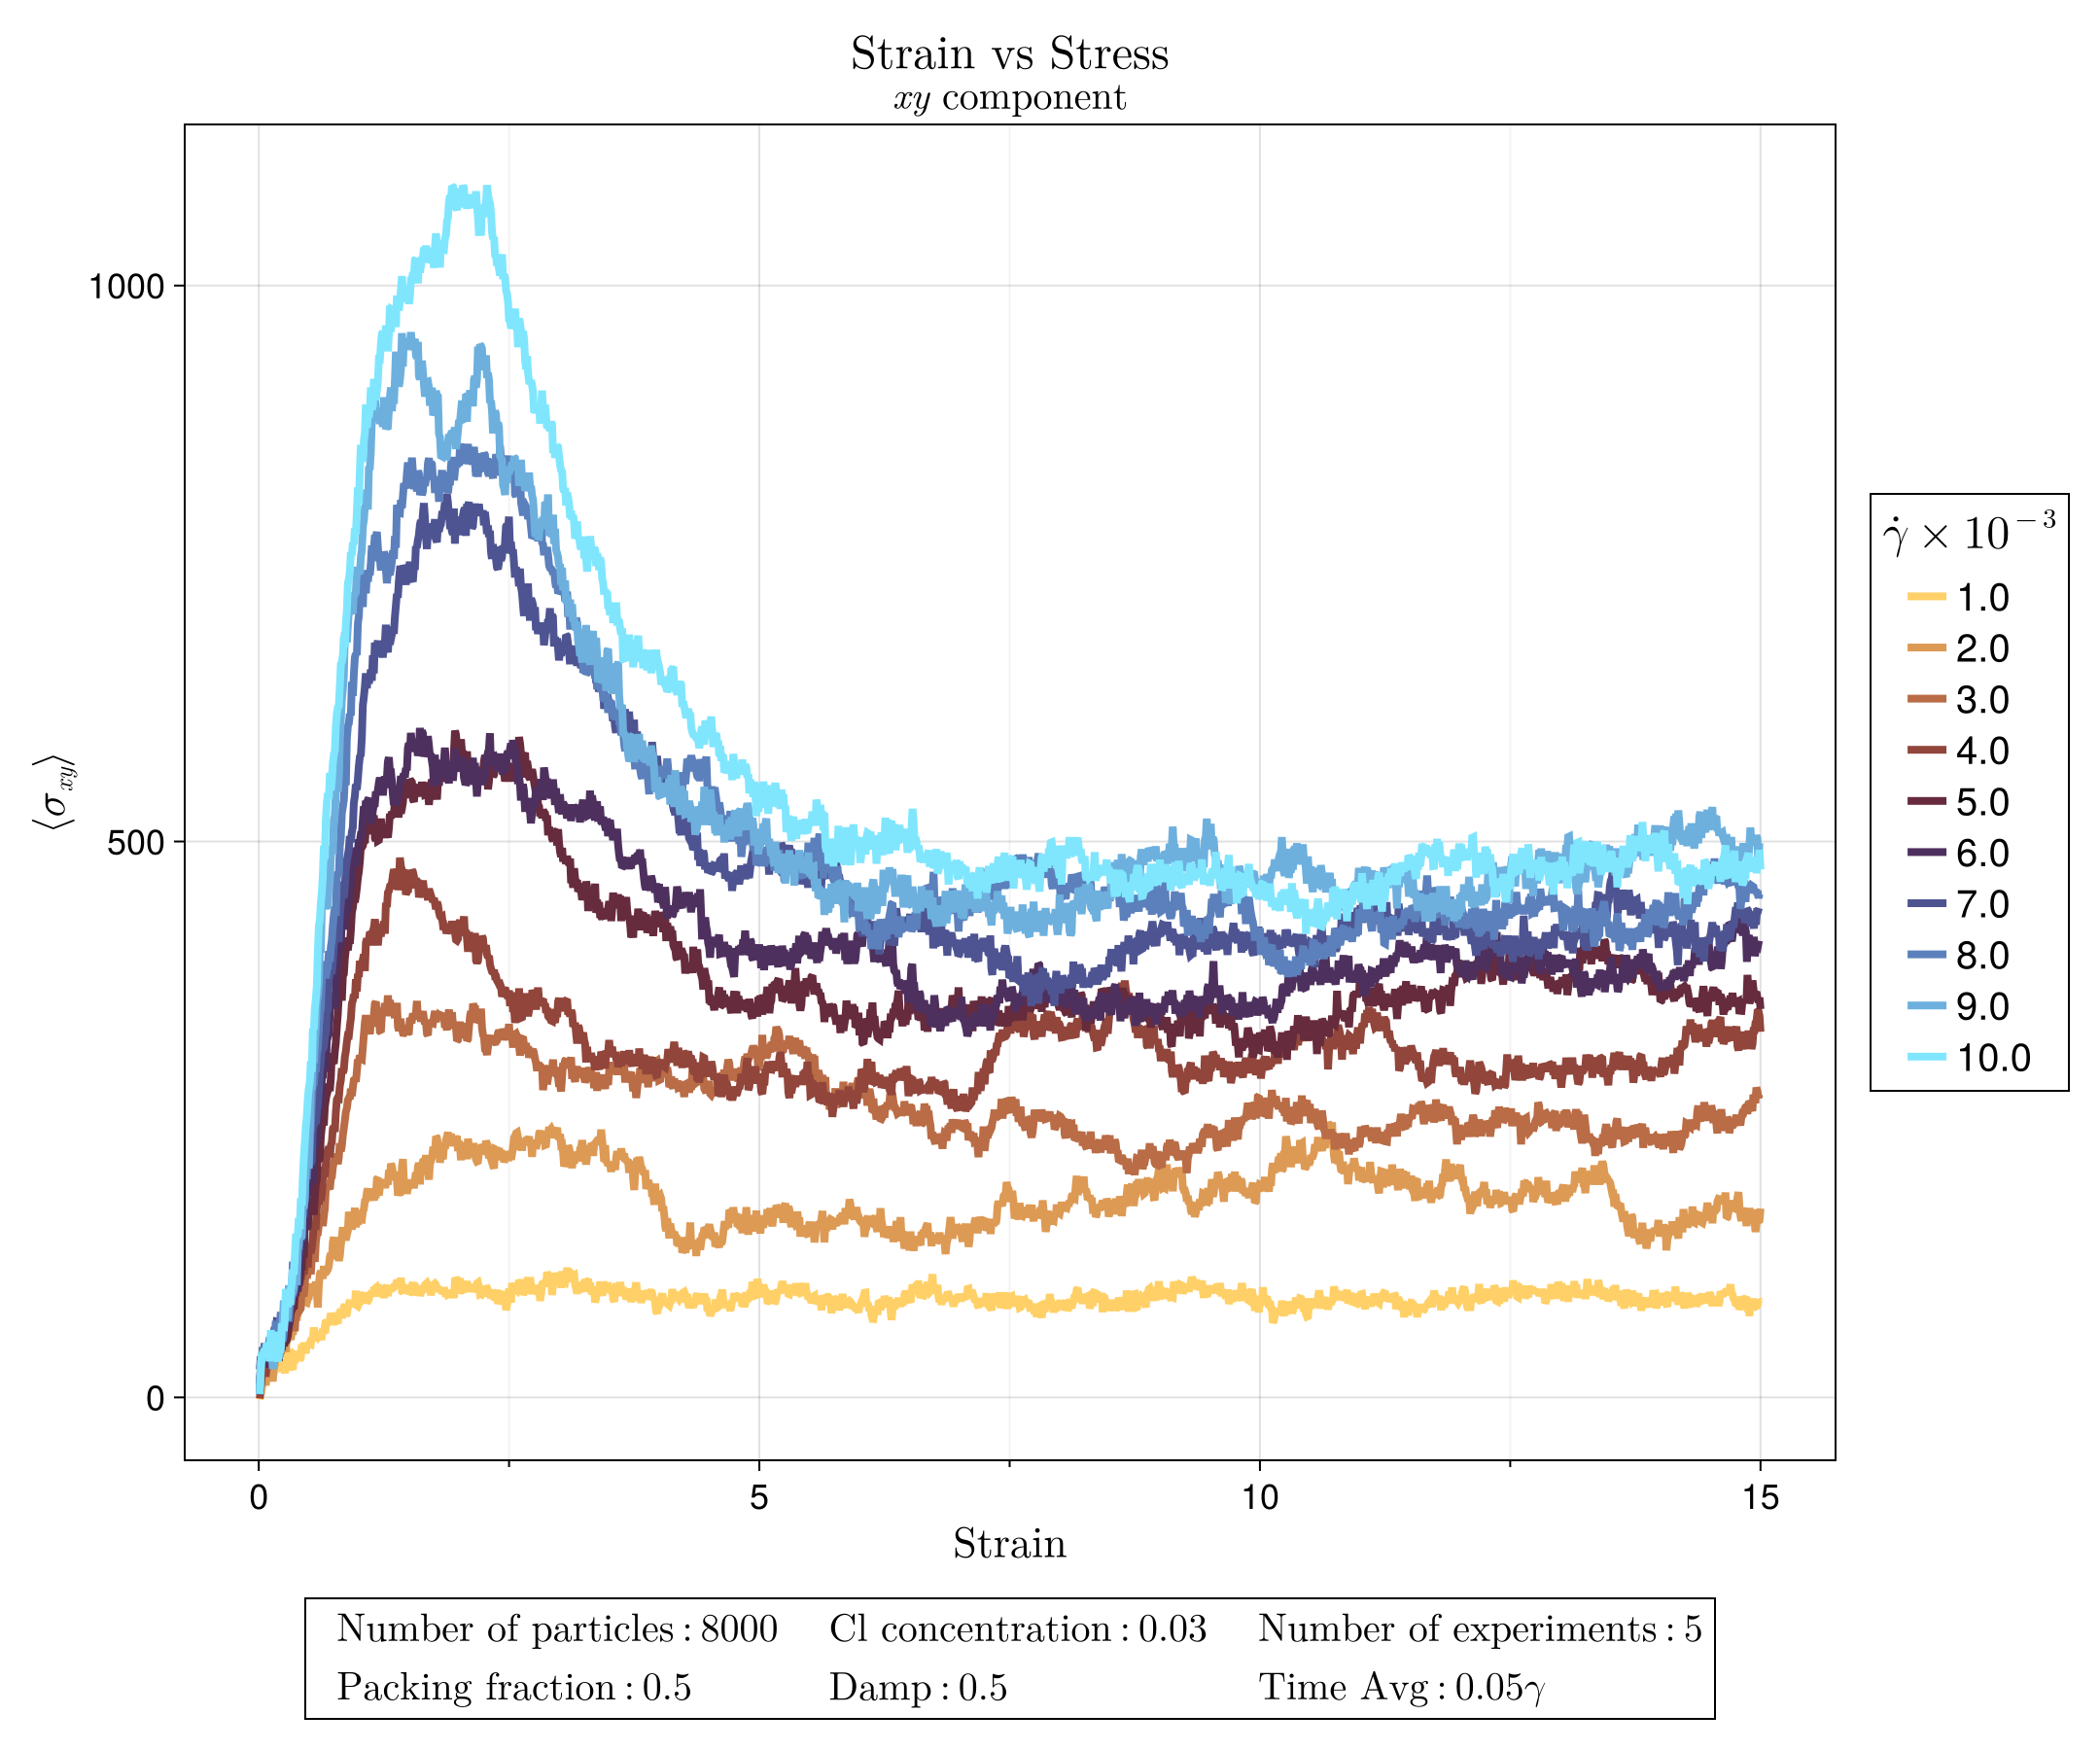
\includegraphics[width=\textwidth]{figs/ComputaitonalResults/CL3/StrainStressXY.png}
    \caption{Stress of a polymeric network with 3\%}
\end{figure}

\begin{figure}[ht!]
    \centering
    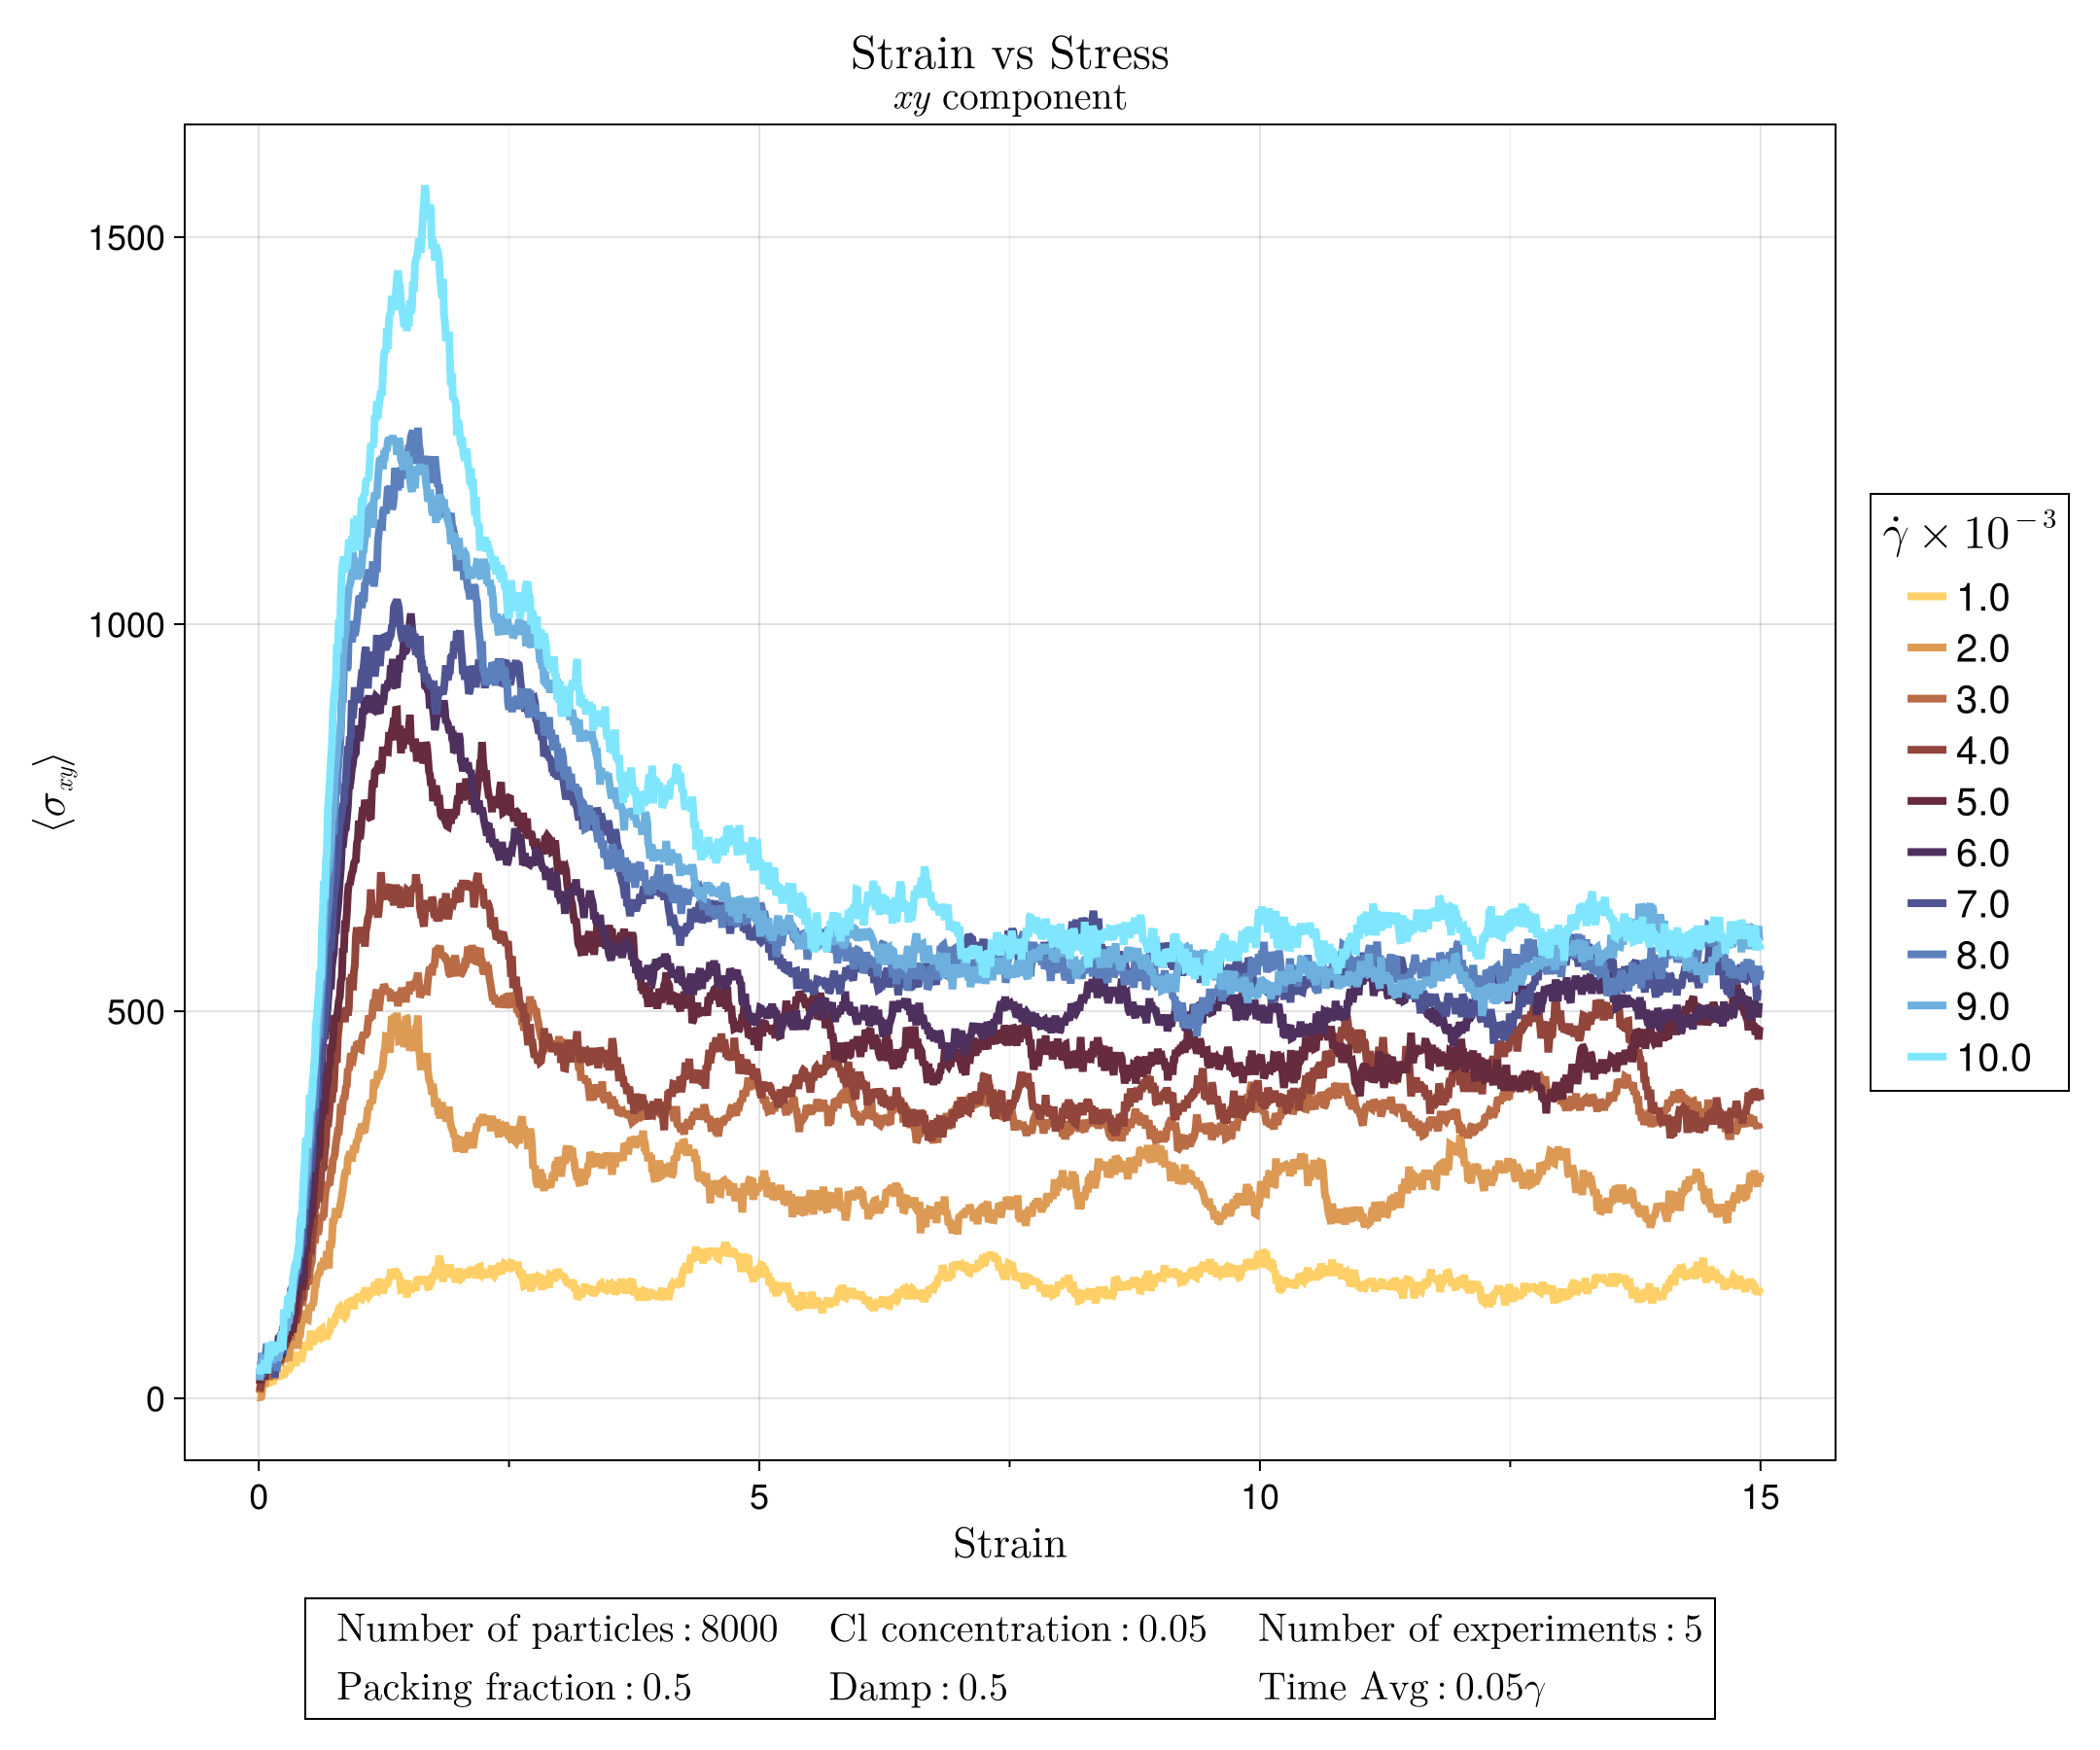
\includegraphics[width=\textwidth]{figs/ComputaitonalResults/CL5/StrainStressXY.png}
    \caption{Stress of a polymeric network with 5\%}
\end{figure}

\begin{figure}[ht!]
    \centering
    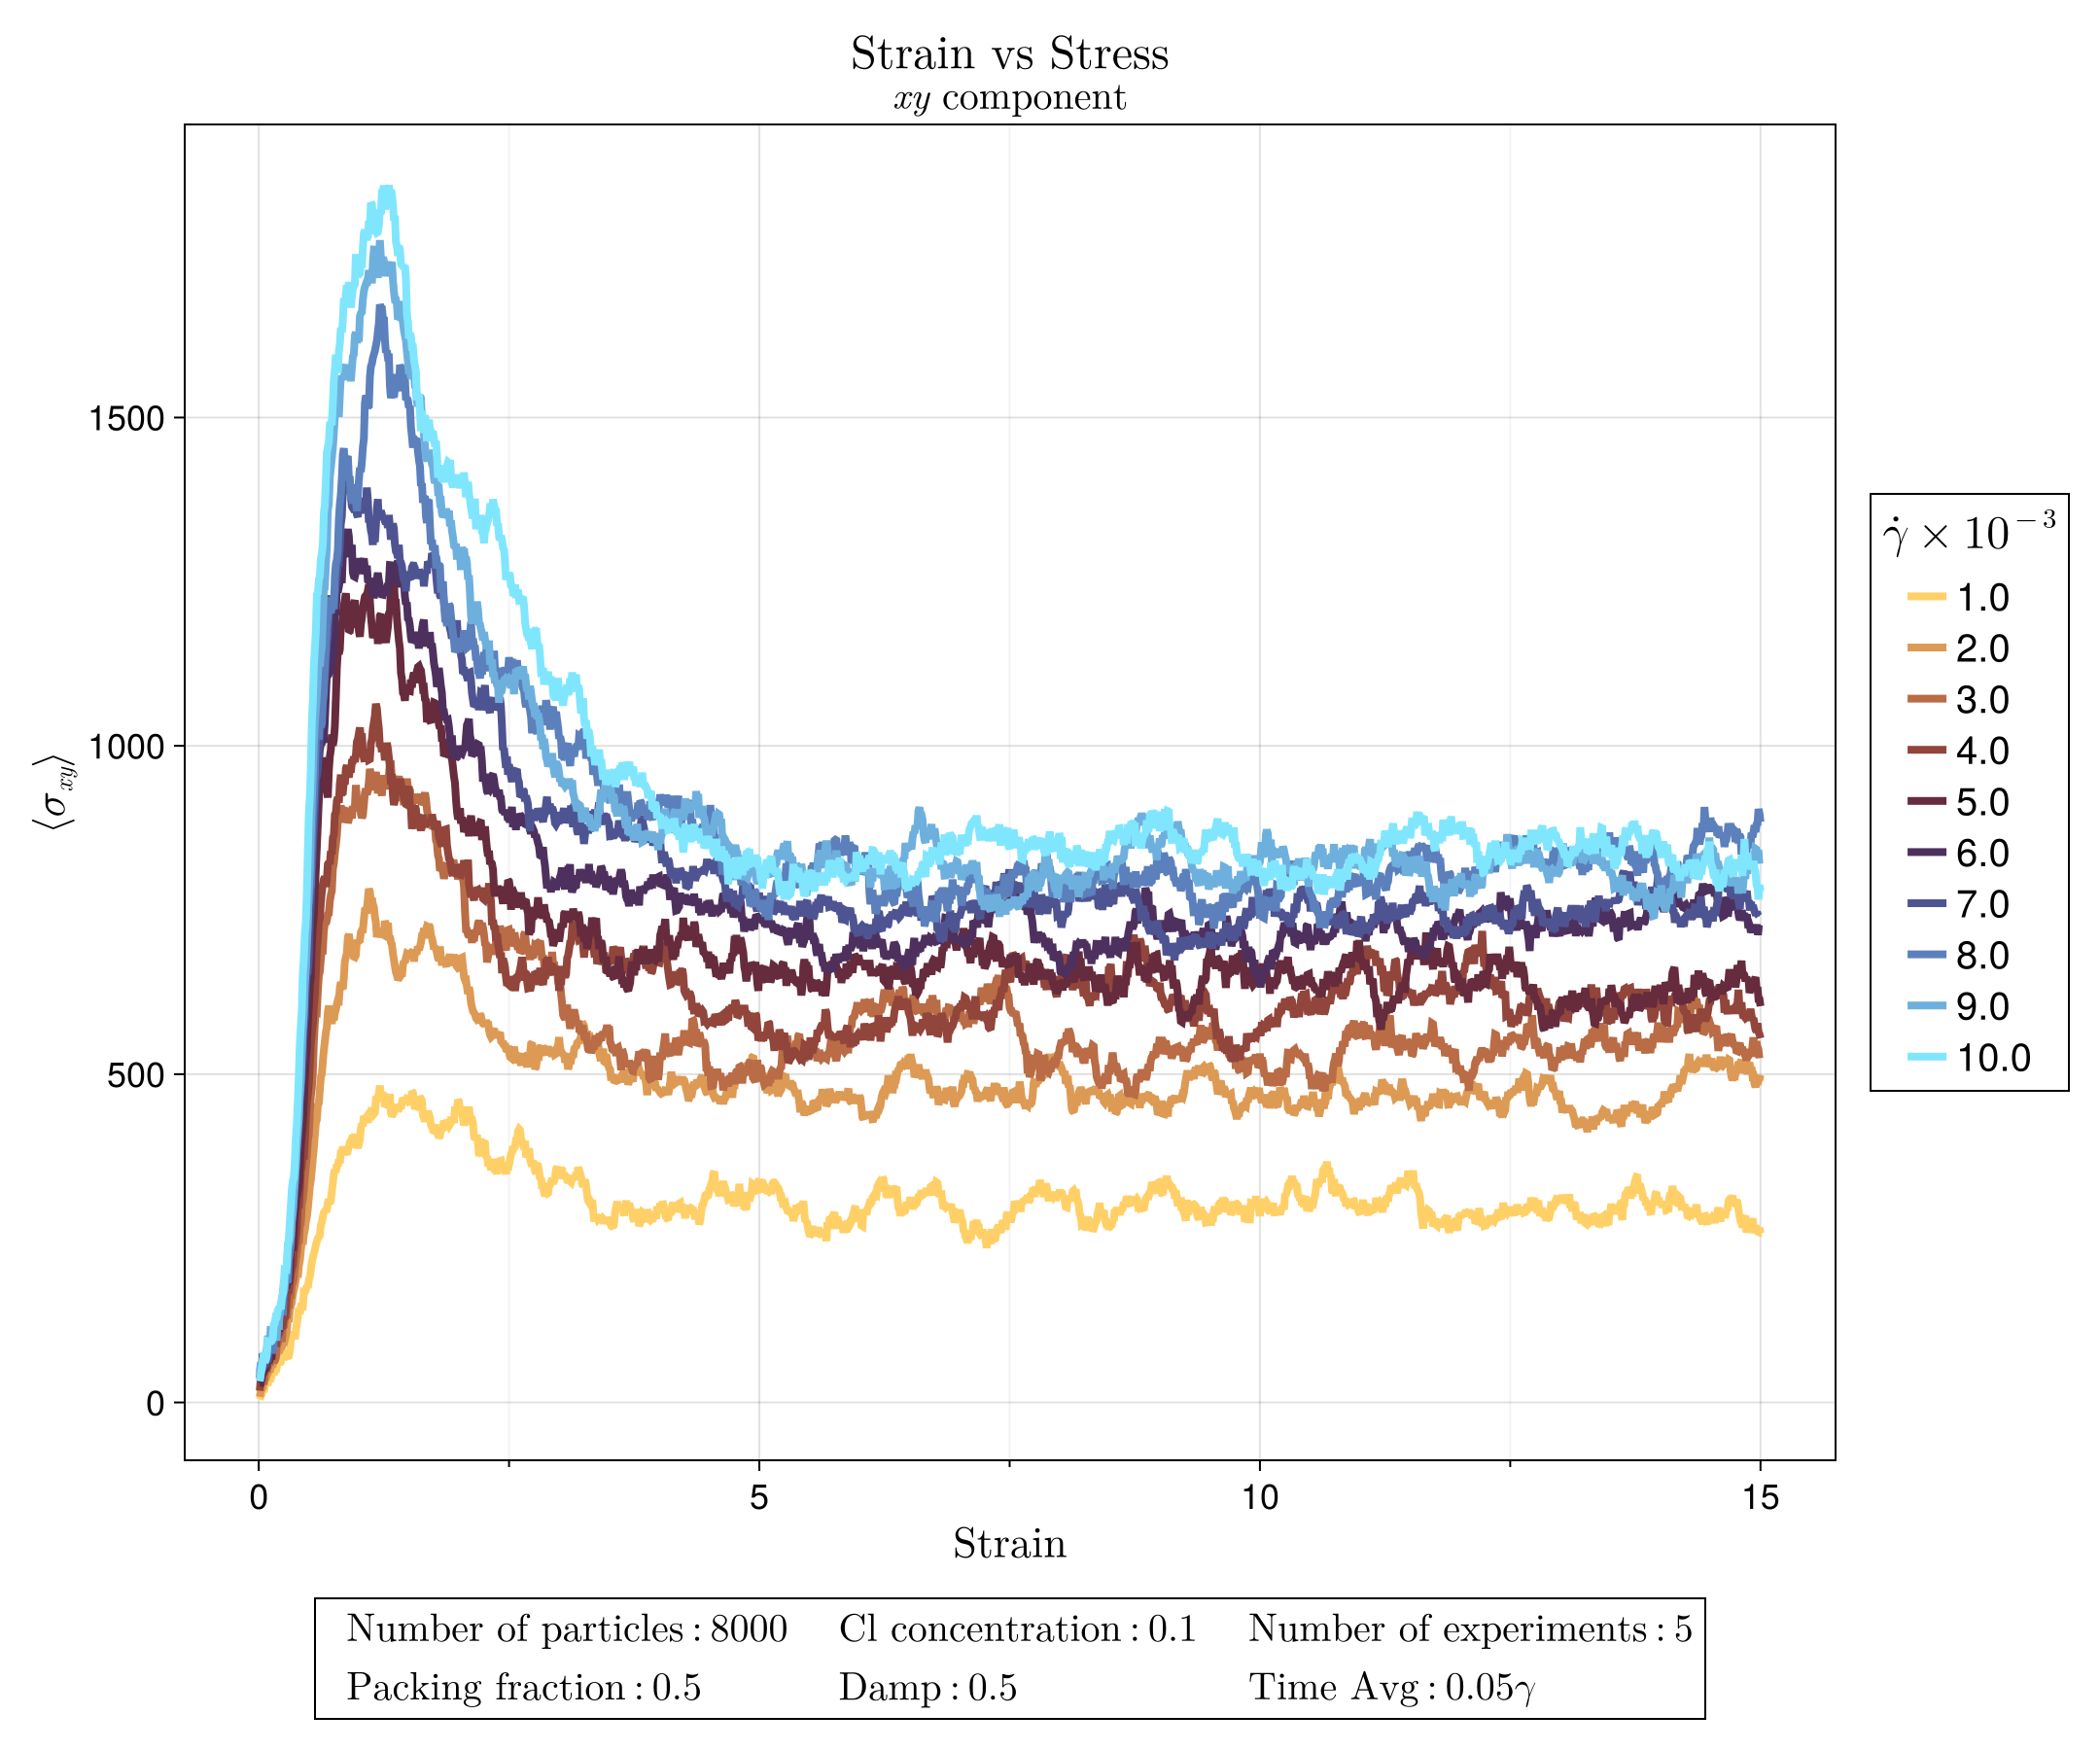
\includegraphics[width=\textwidth]{figs/ComputaitonalResults/CL10/StrainStressXY.png}
    \caption{Stress of a polymeric network with 10\%}
\end{figure}

\begin{figure}[ht!]
    \centering
    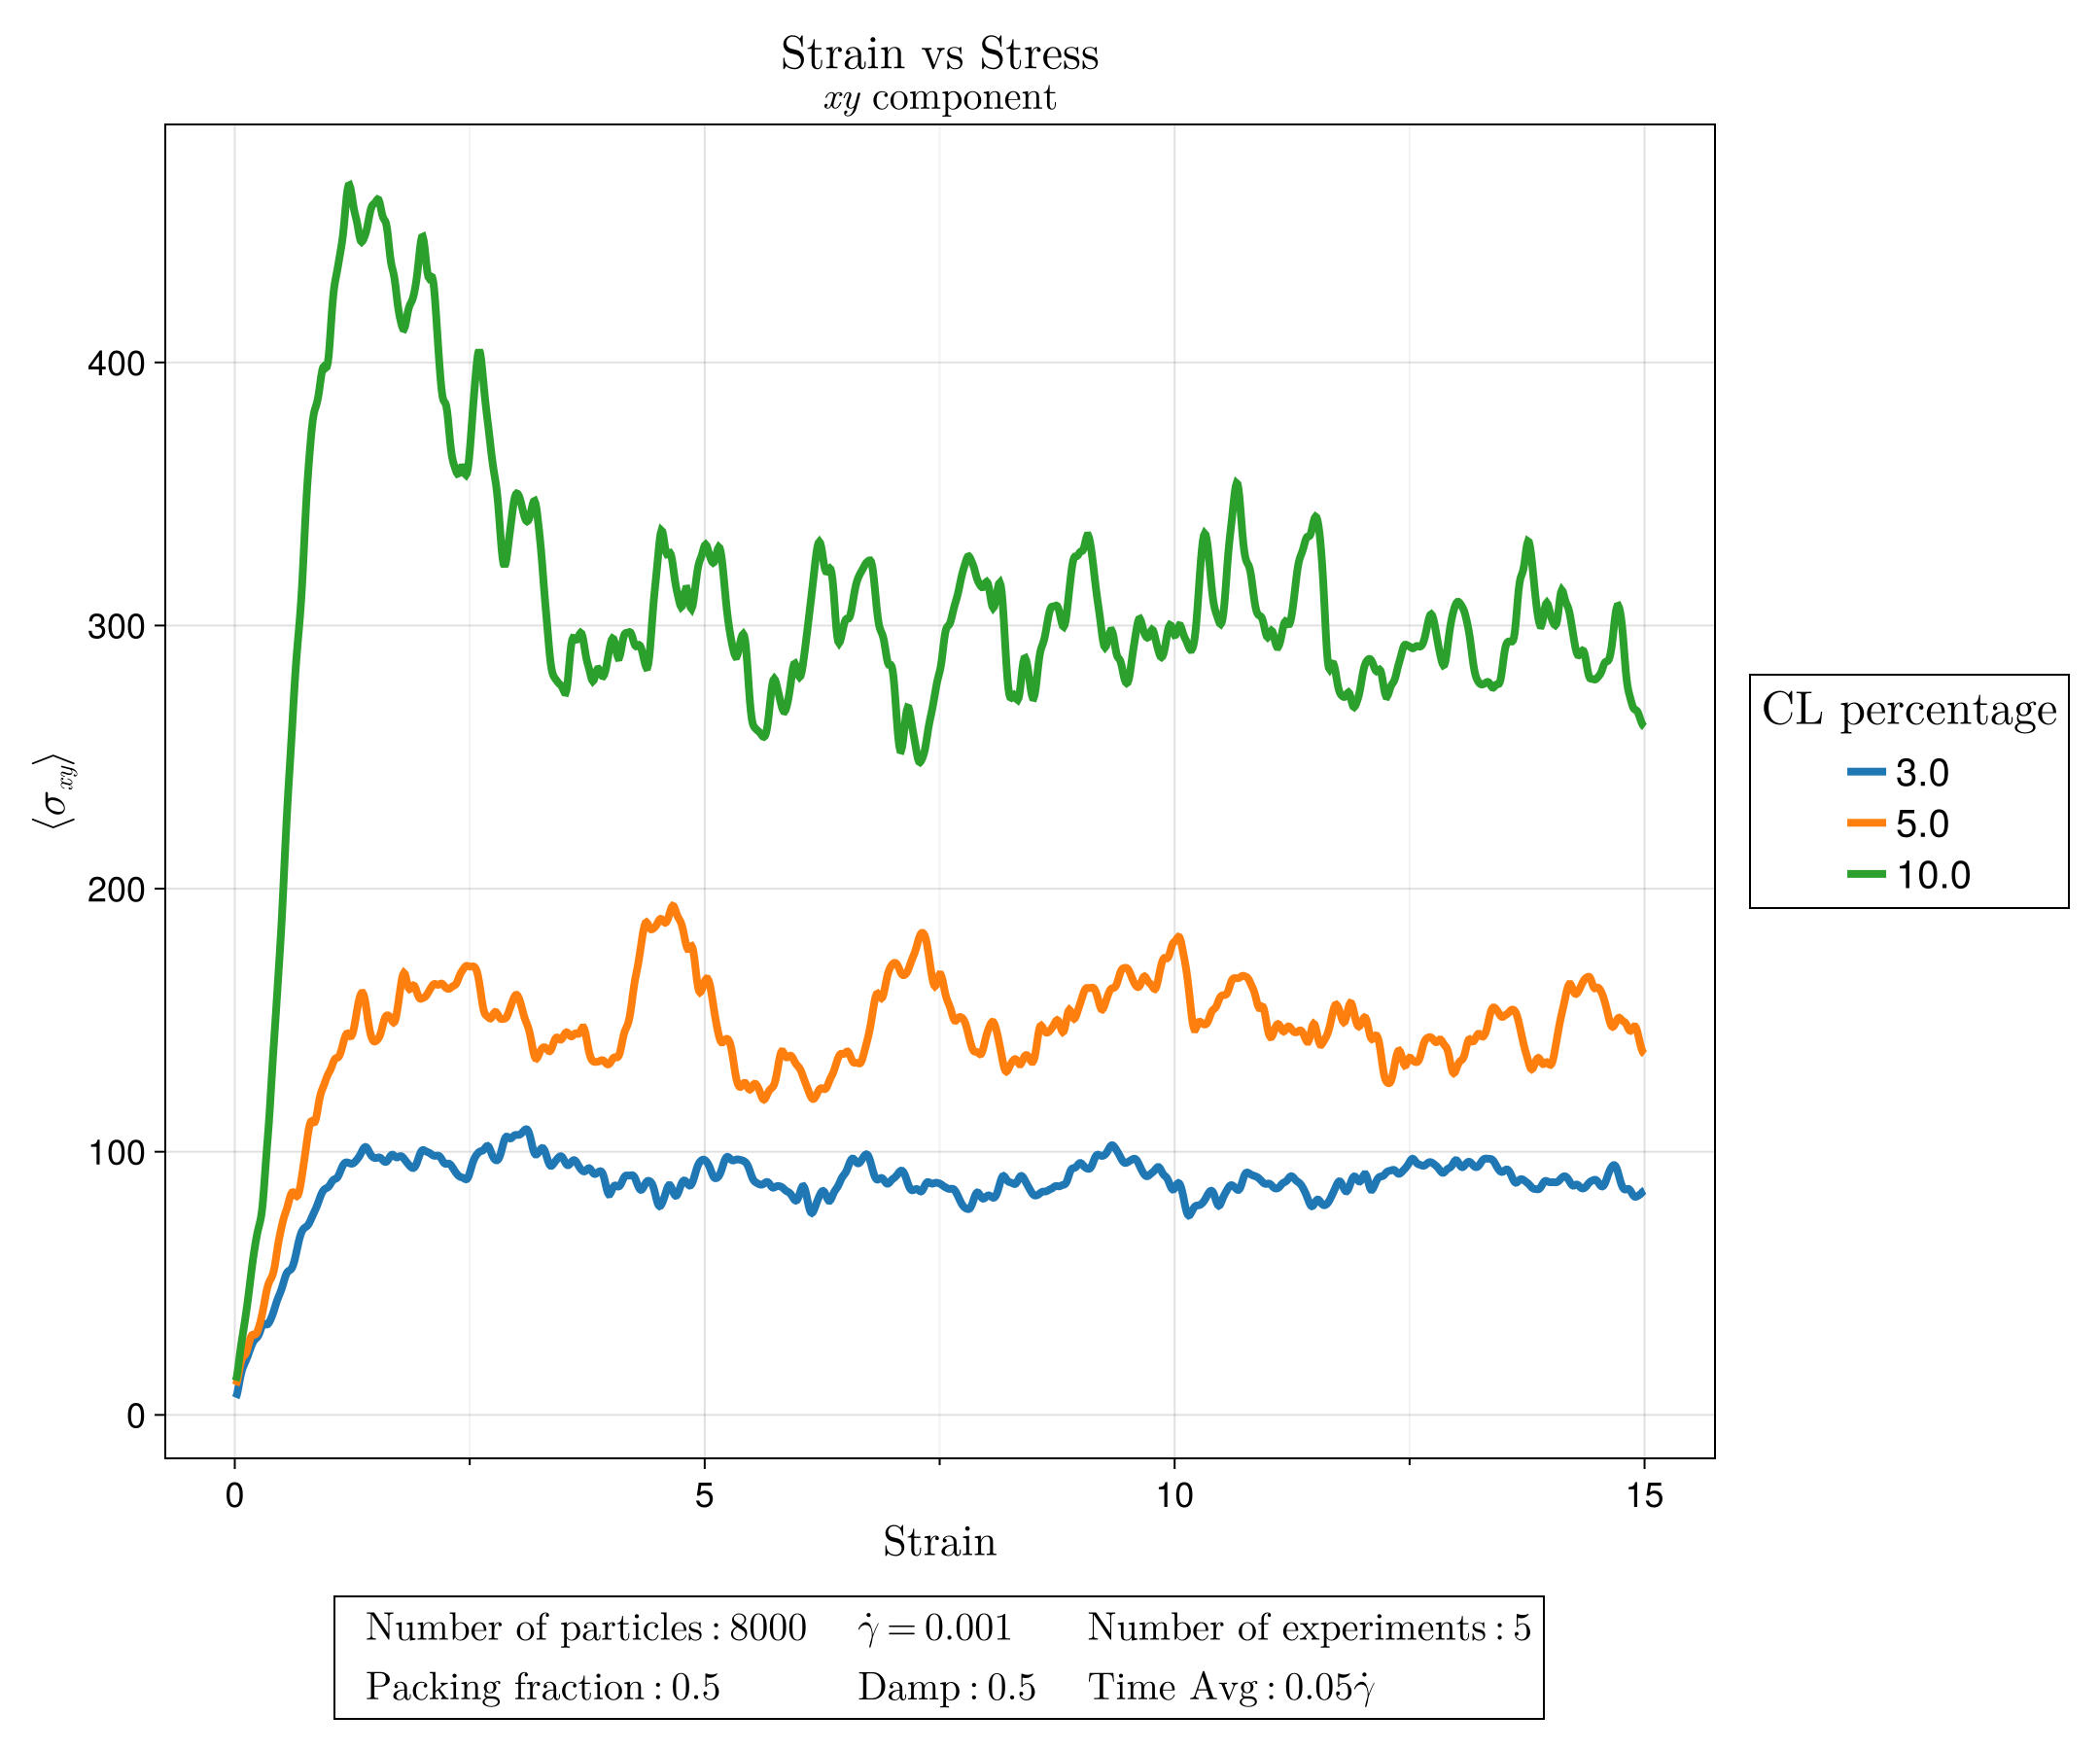
\includegraphics[width=\textwidth]{figs/ComputaitonalResults/dgamma1Stress.png}
    \caption{Stress for different polymeric network at shear rate of \num{0.001}}
\end{figure}

\begin{figure}[ht!]
    \centering
    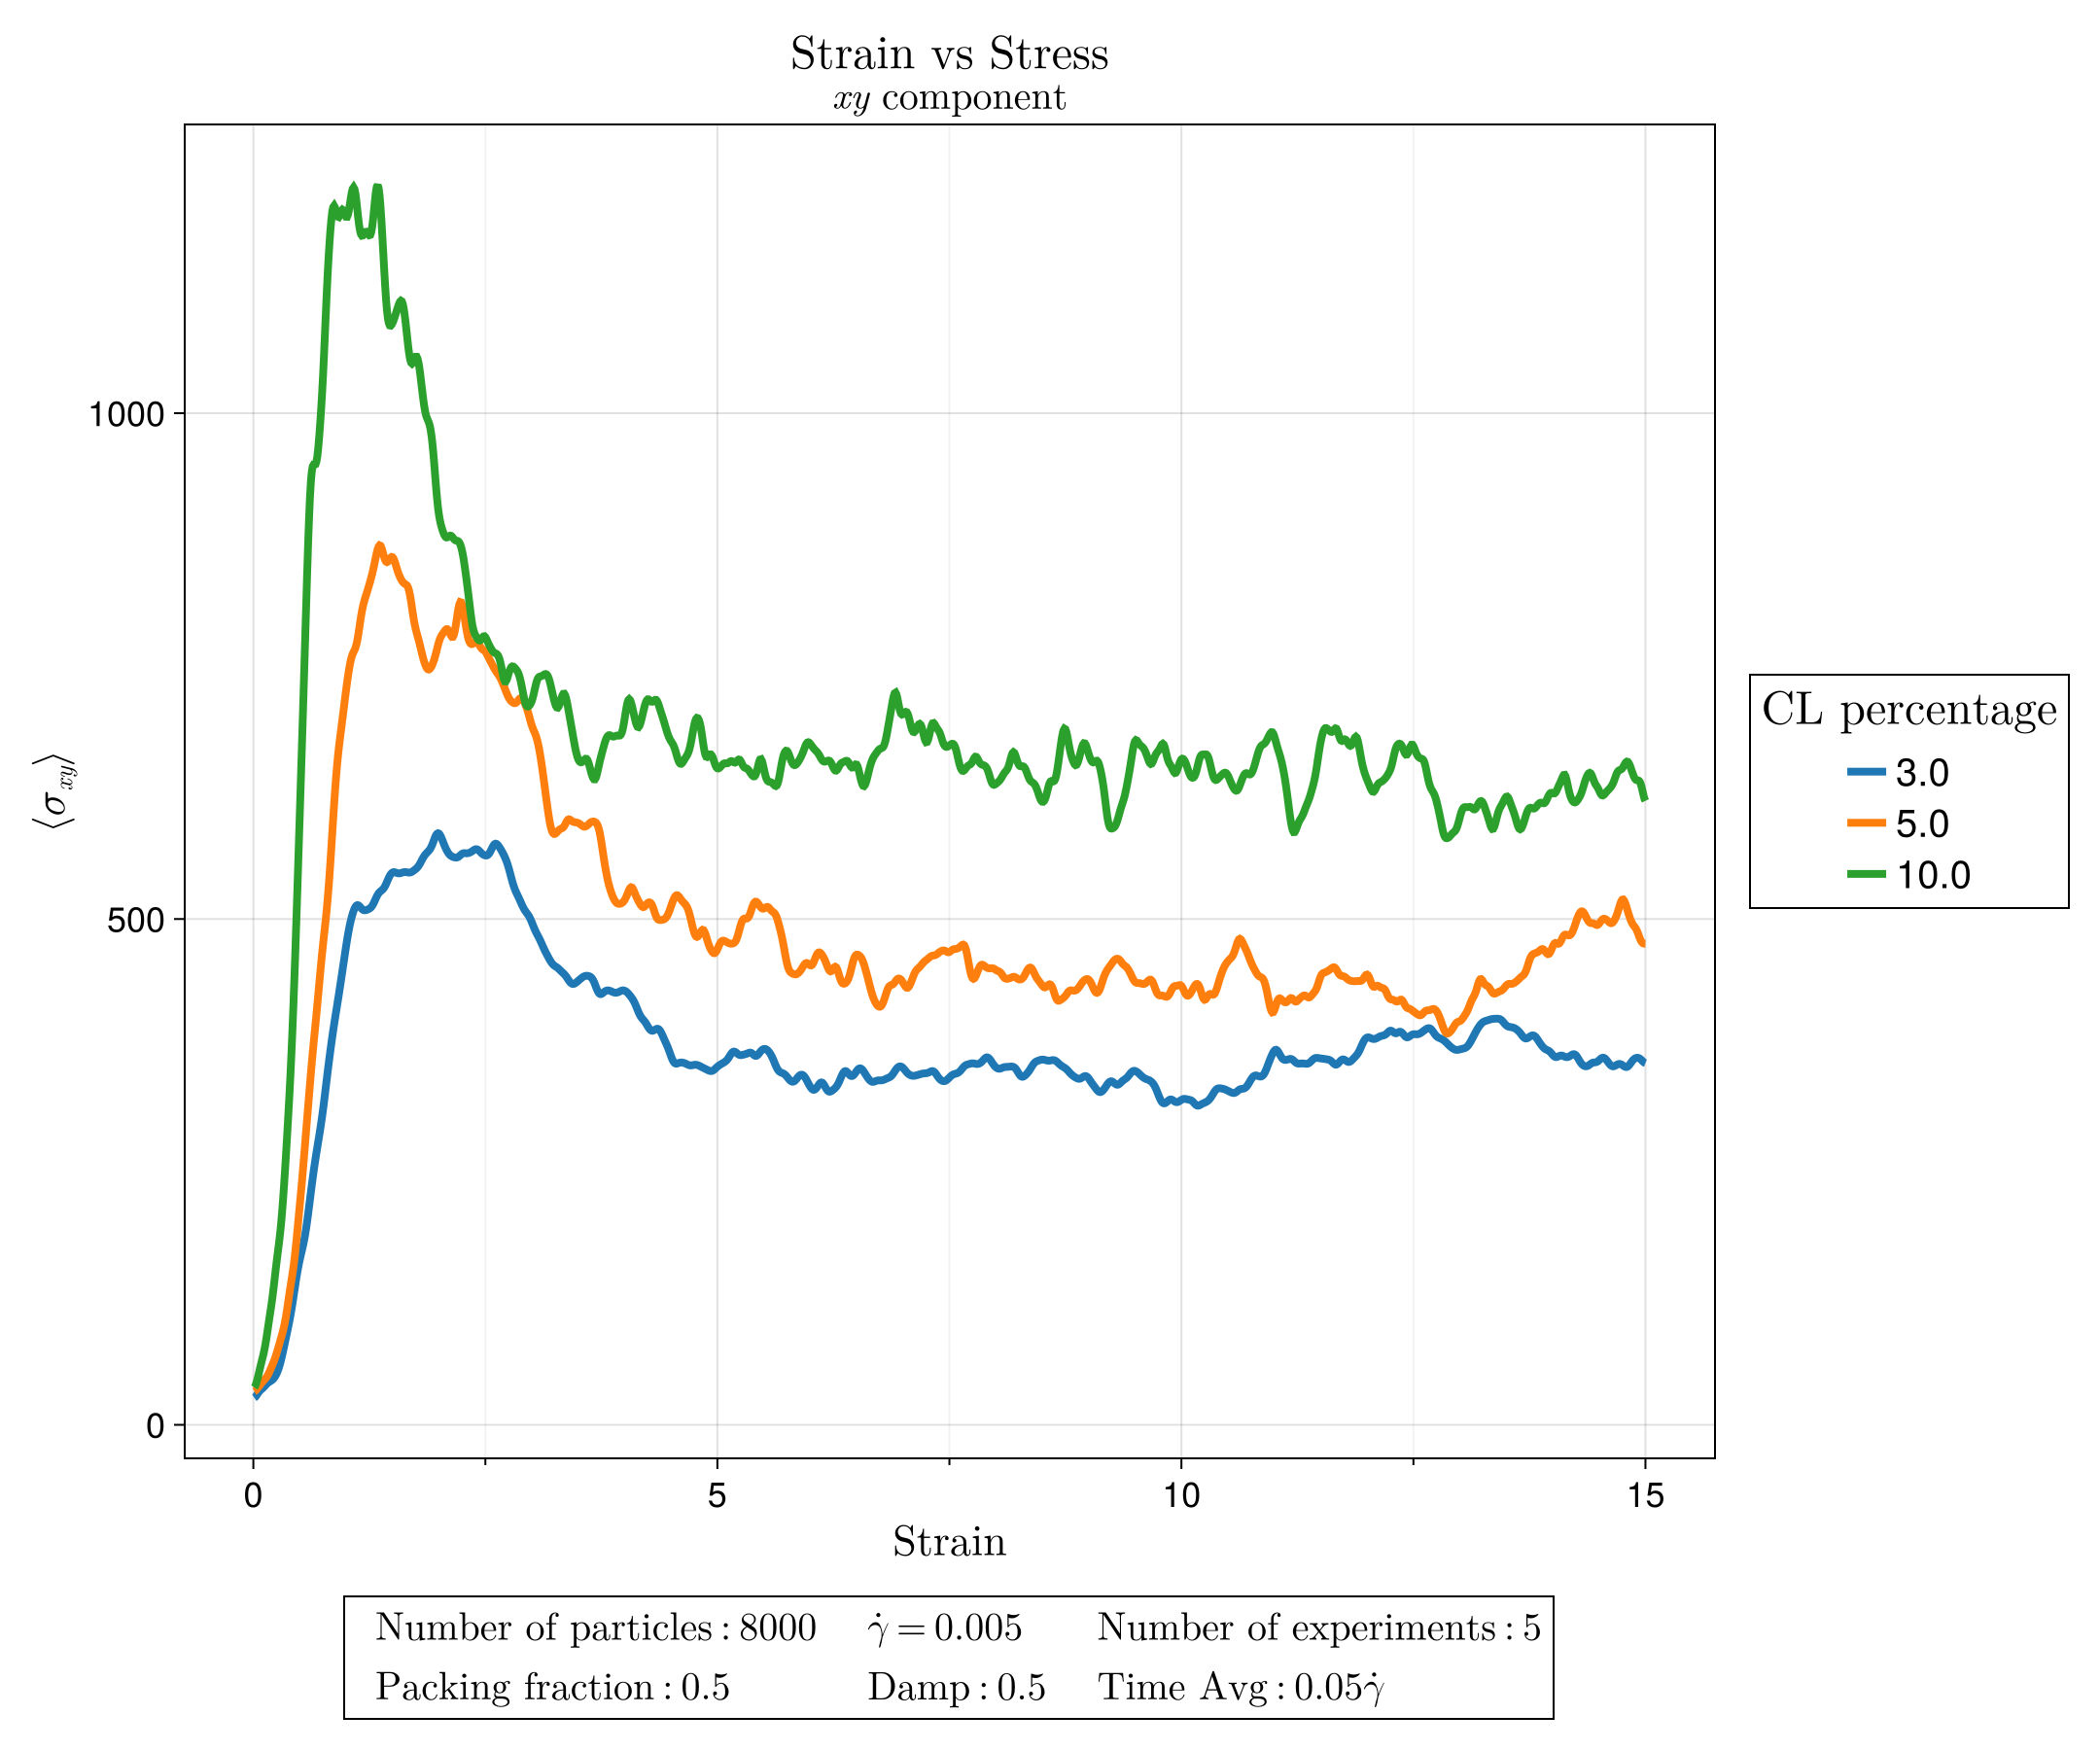
\includegraphics[width=\textwidth]{figs/ComputaitonalResults/dgamma5Stress.png}
    \caption{Stress for different polymeric network at shear rate of \num{0.005}}
\end{figure}

\begin{figure}[ht!]
    \centering
    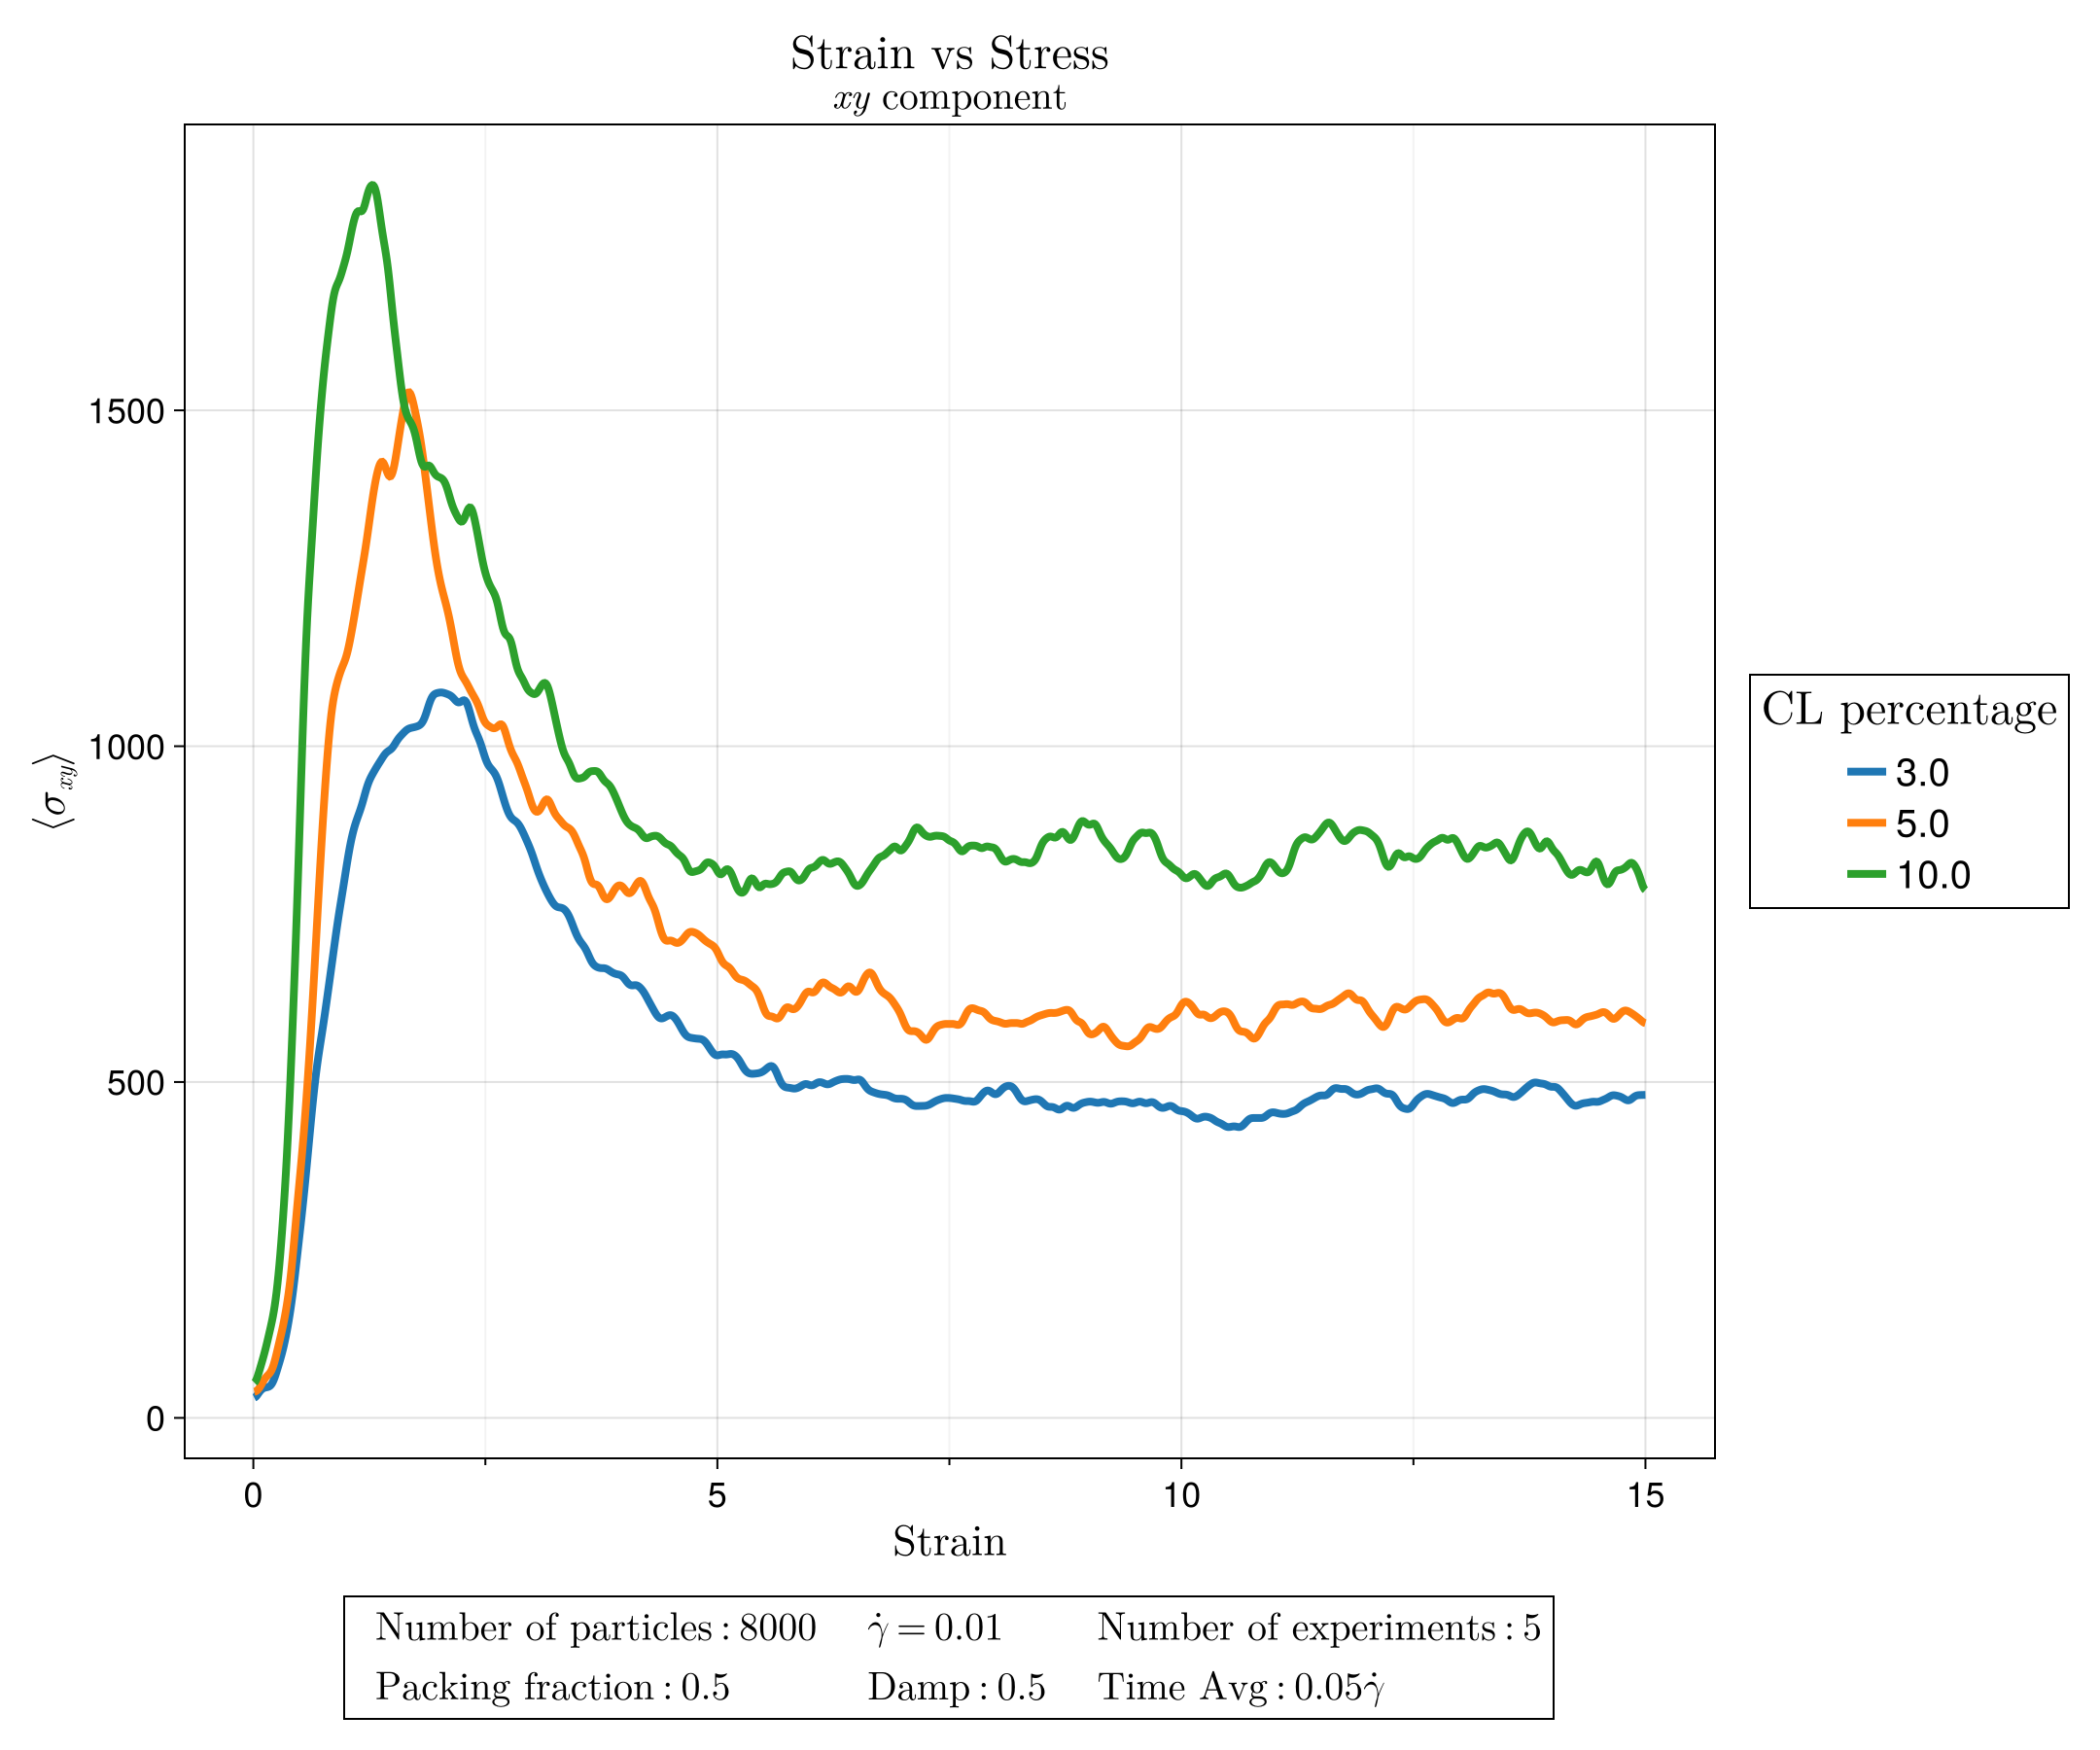
\includegraphics[width=\textwidth]{figs/ComputaitonalResults/dgamma10Stress.png}
    \caption{Stress for different polymeric network at shear rate of \num{0.01}}
\end{figure}


\begin{figure}[ht!]
    \centering
    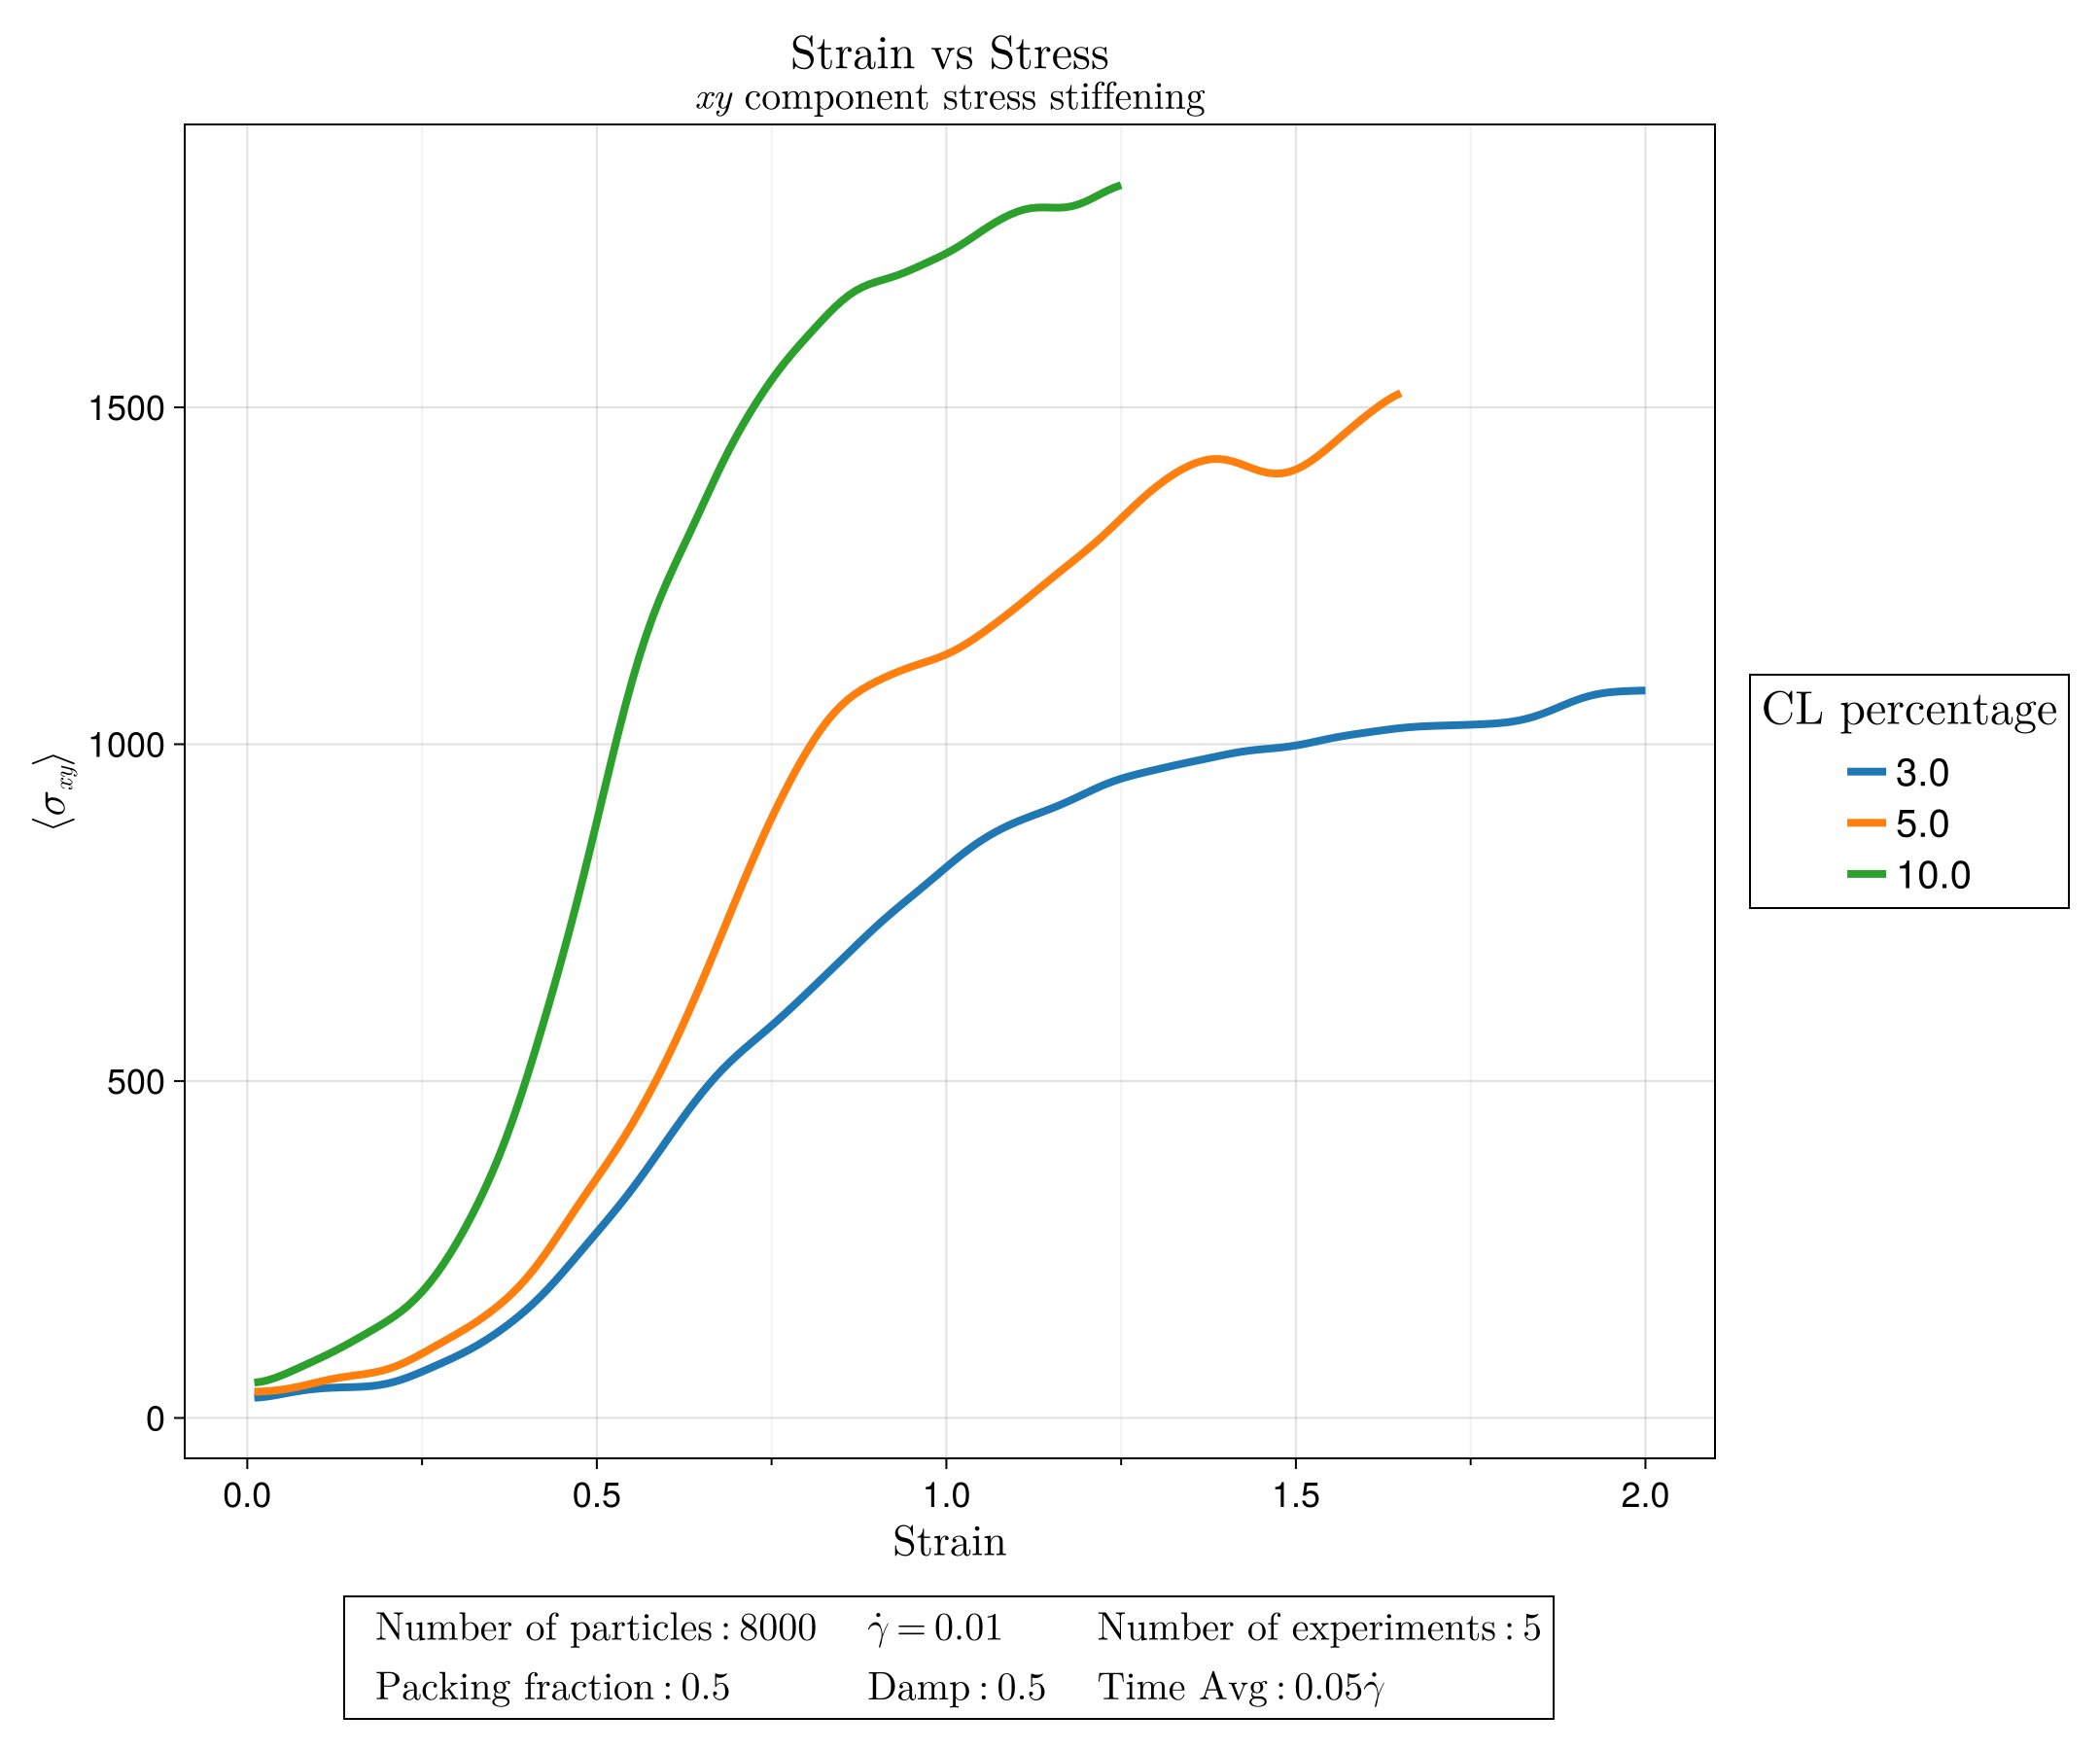
\includegraphics[width=\textwidth]{figs/ComputaitonalResults/stiff_dgamma10Stress.png}
    \caption{Stress stiffening for a shear rate of \num{0.01} at different crosslinker concentrations.}
\end{figure}

\begin{figure}[ht!]
    \centering
    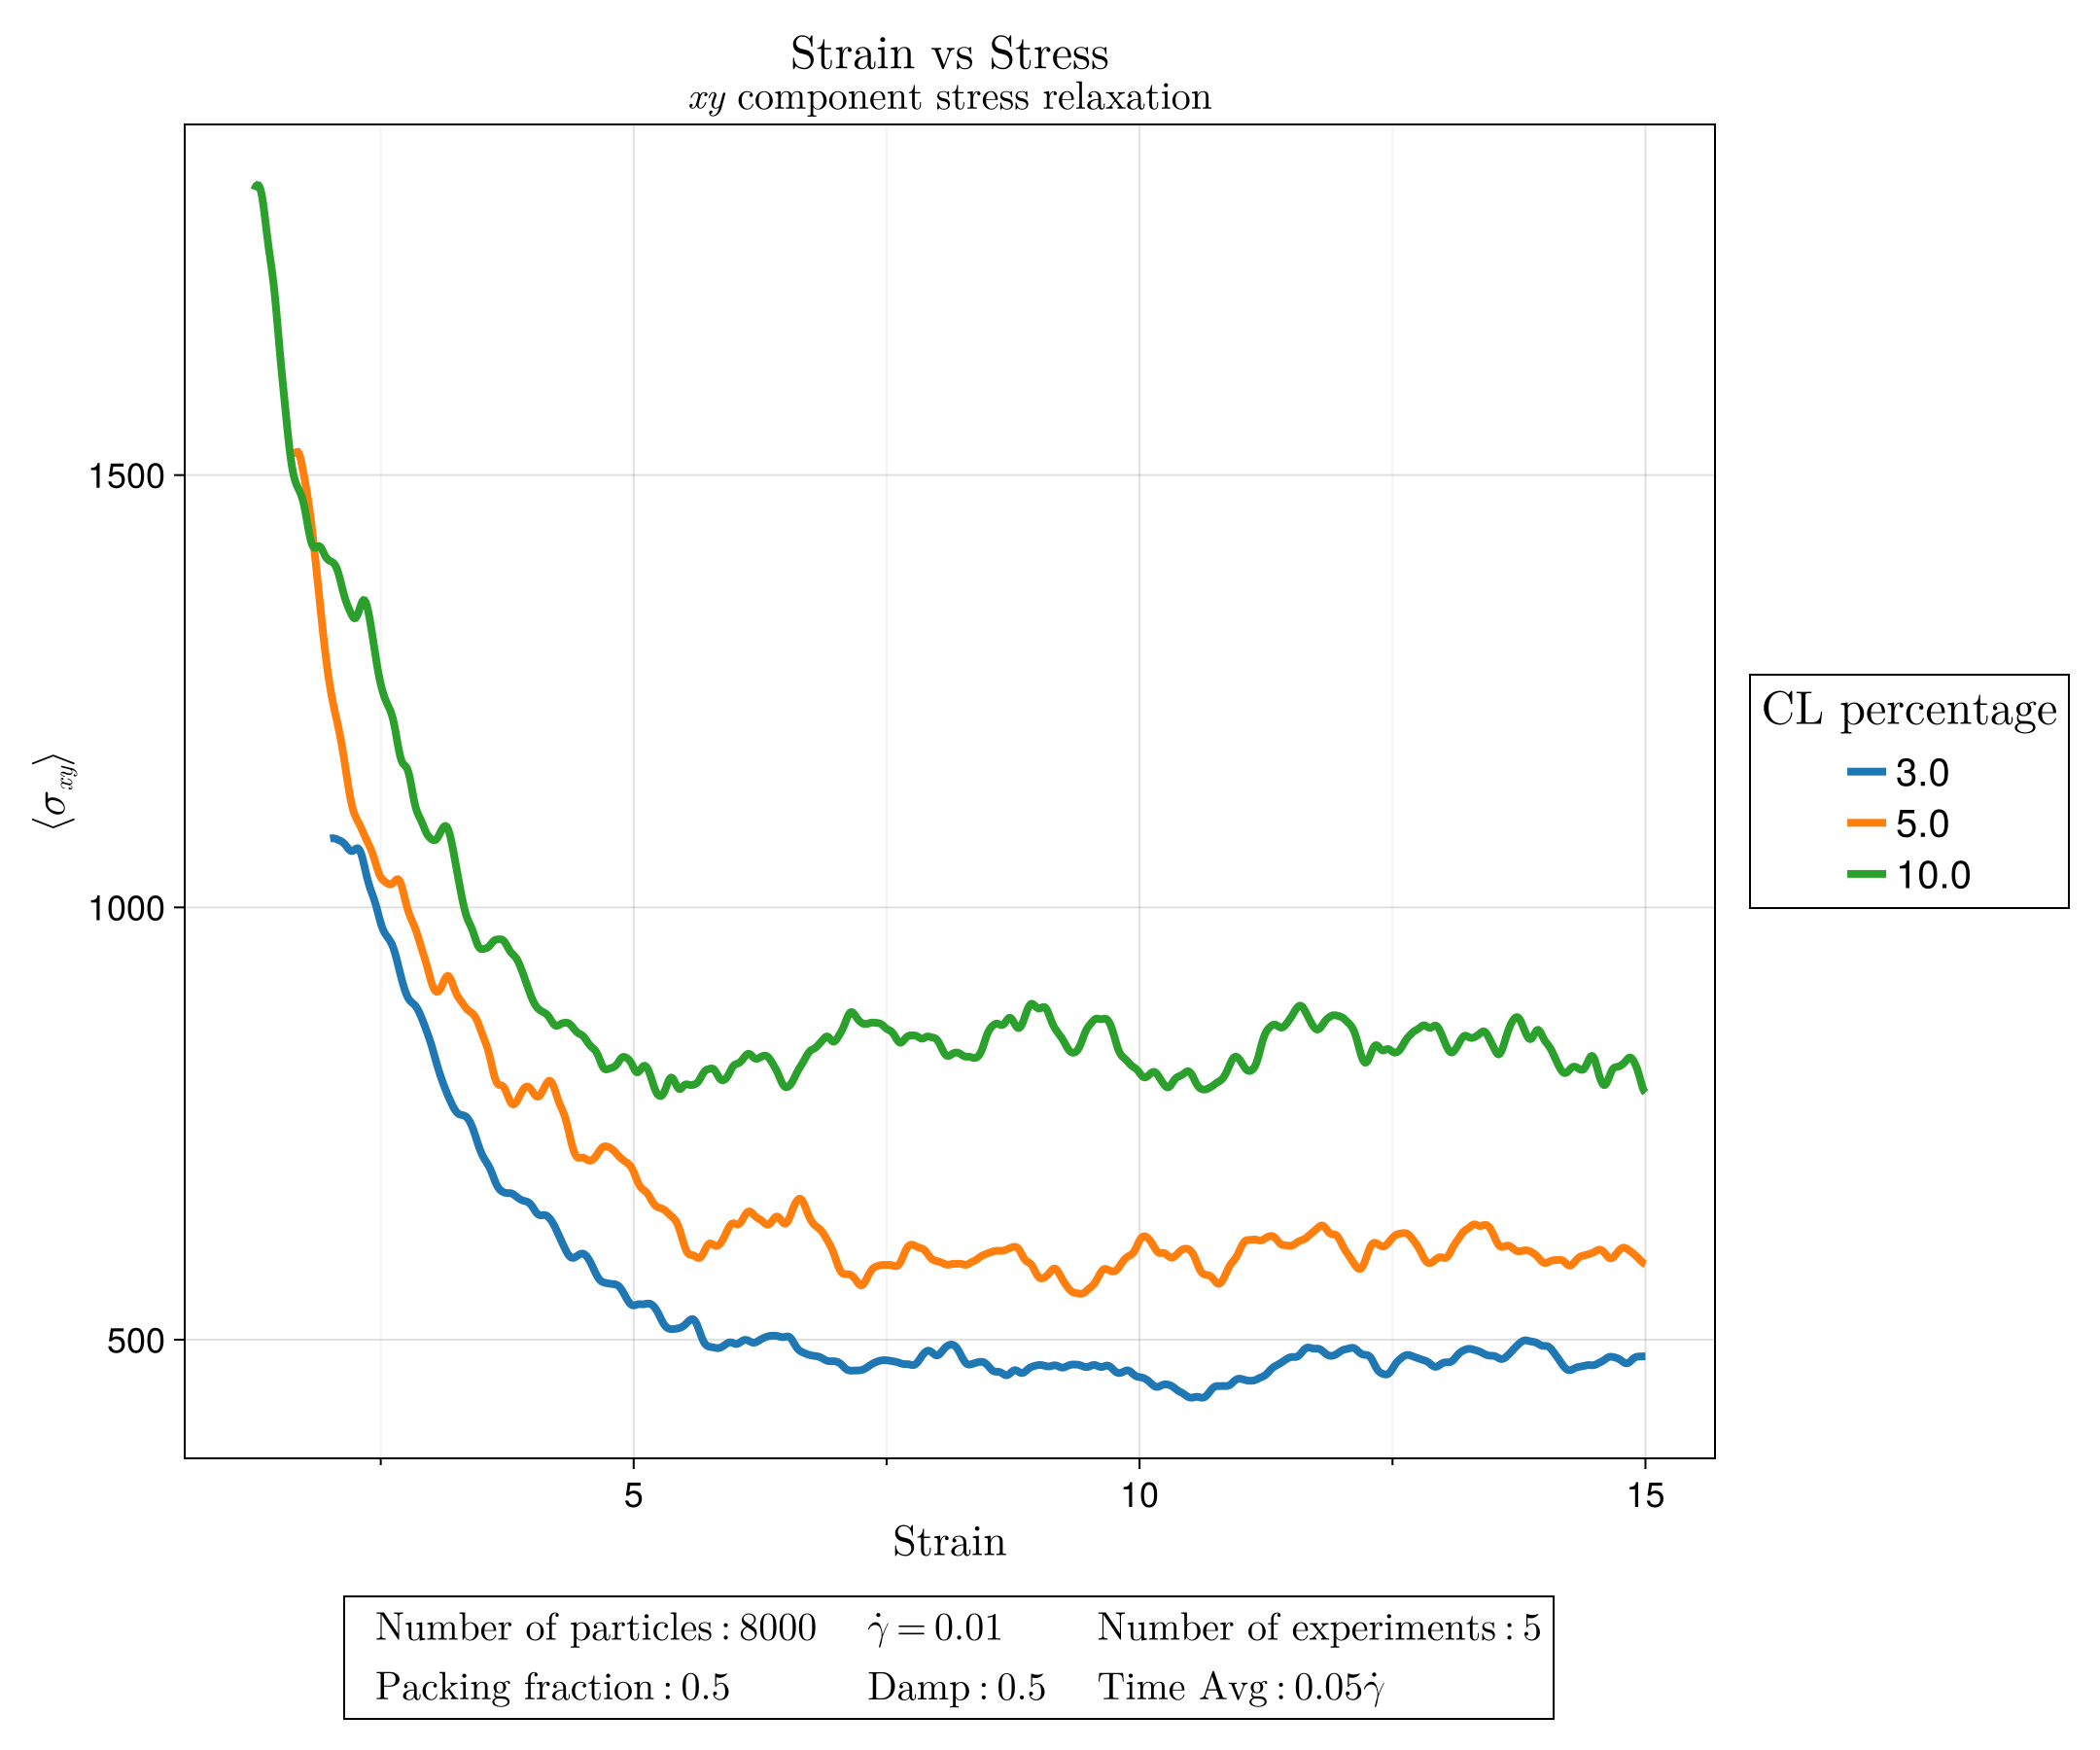
\includegraphics[width=\textwidth]{figs/ComputaitonalResults/srlx_dgamma10Stress.png}
    \caption{Stress relaxation for a shear rate of \num{0.01} at different crosslinker concentrations.}
\end{figure}



\begin{figure}[ht!]
    \centering
    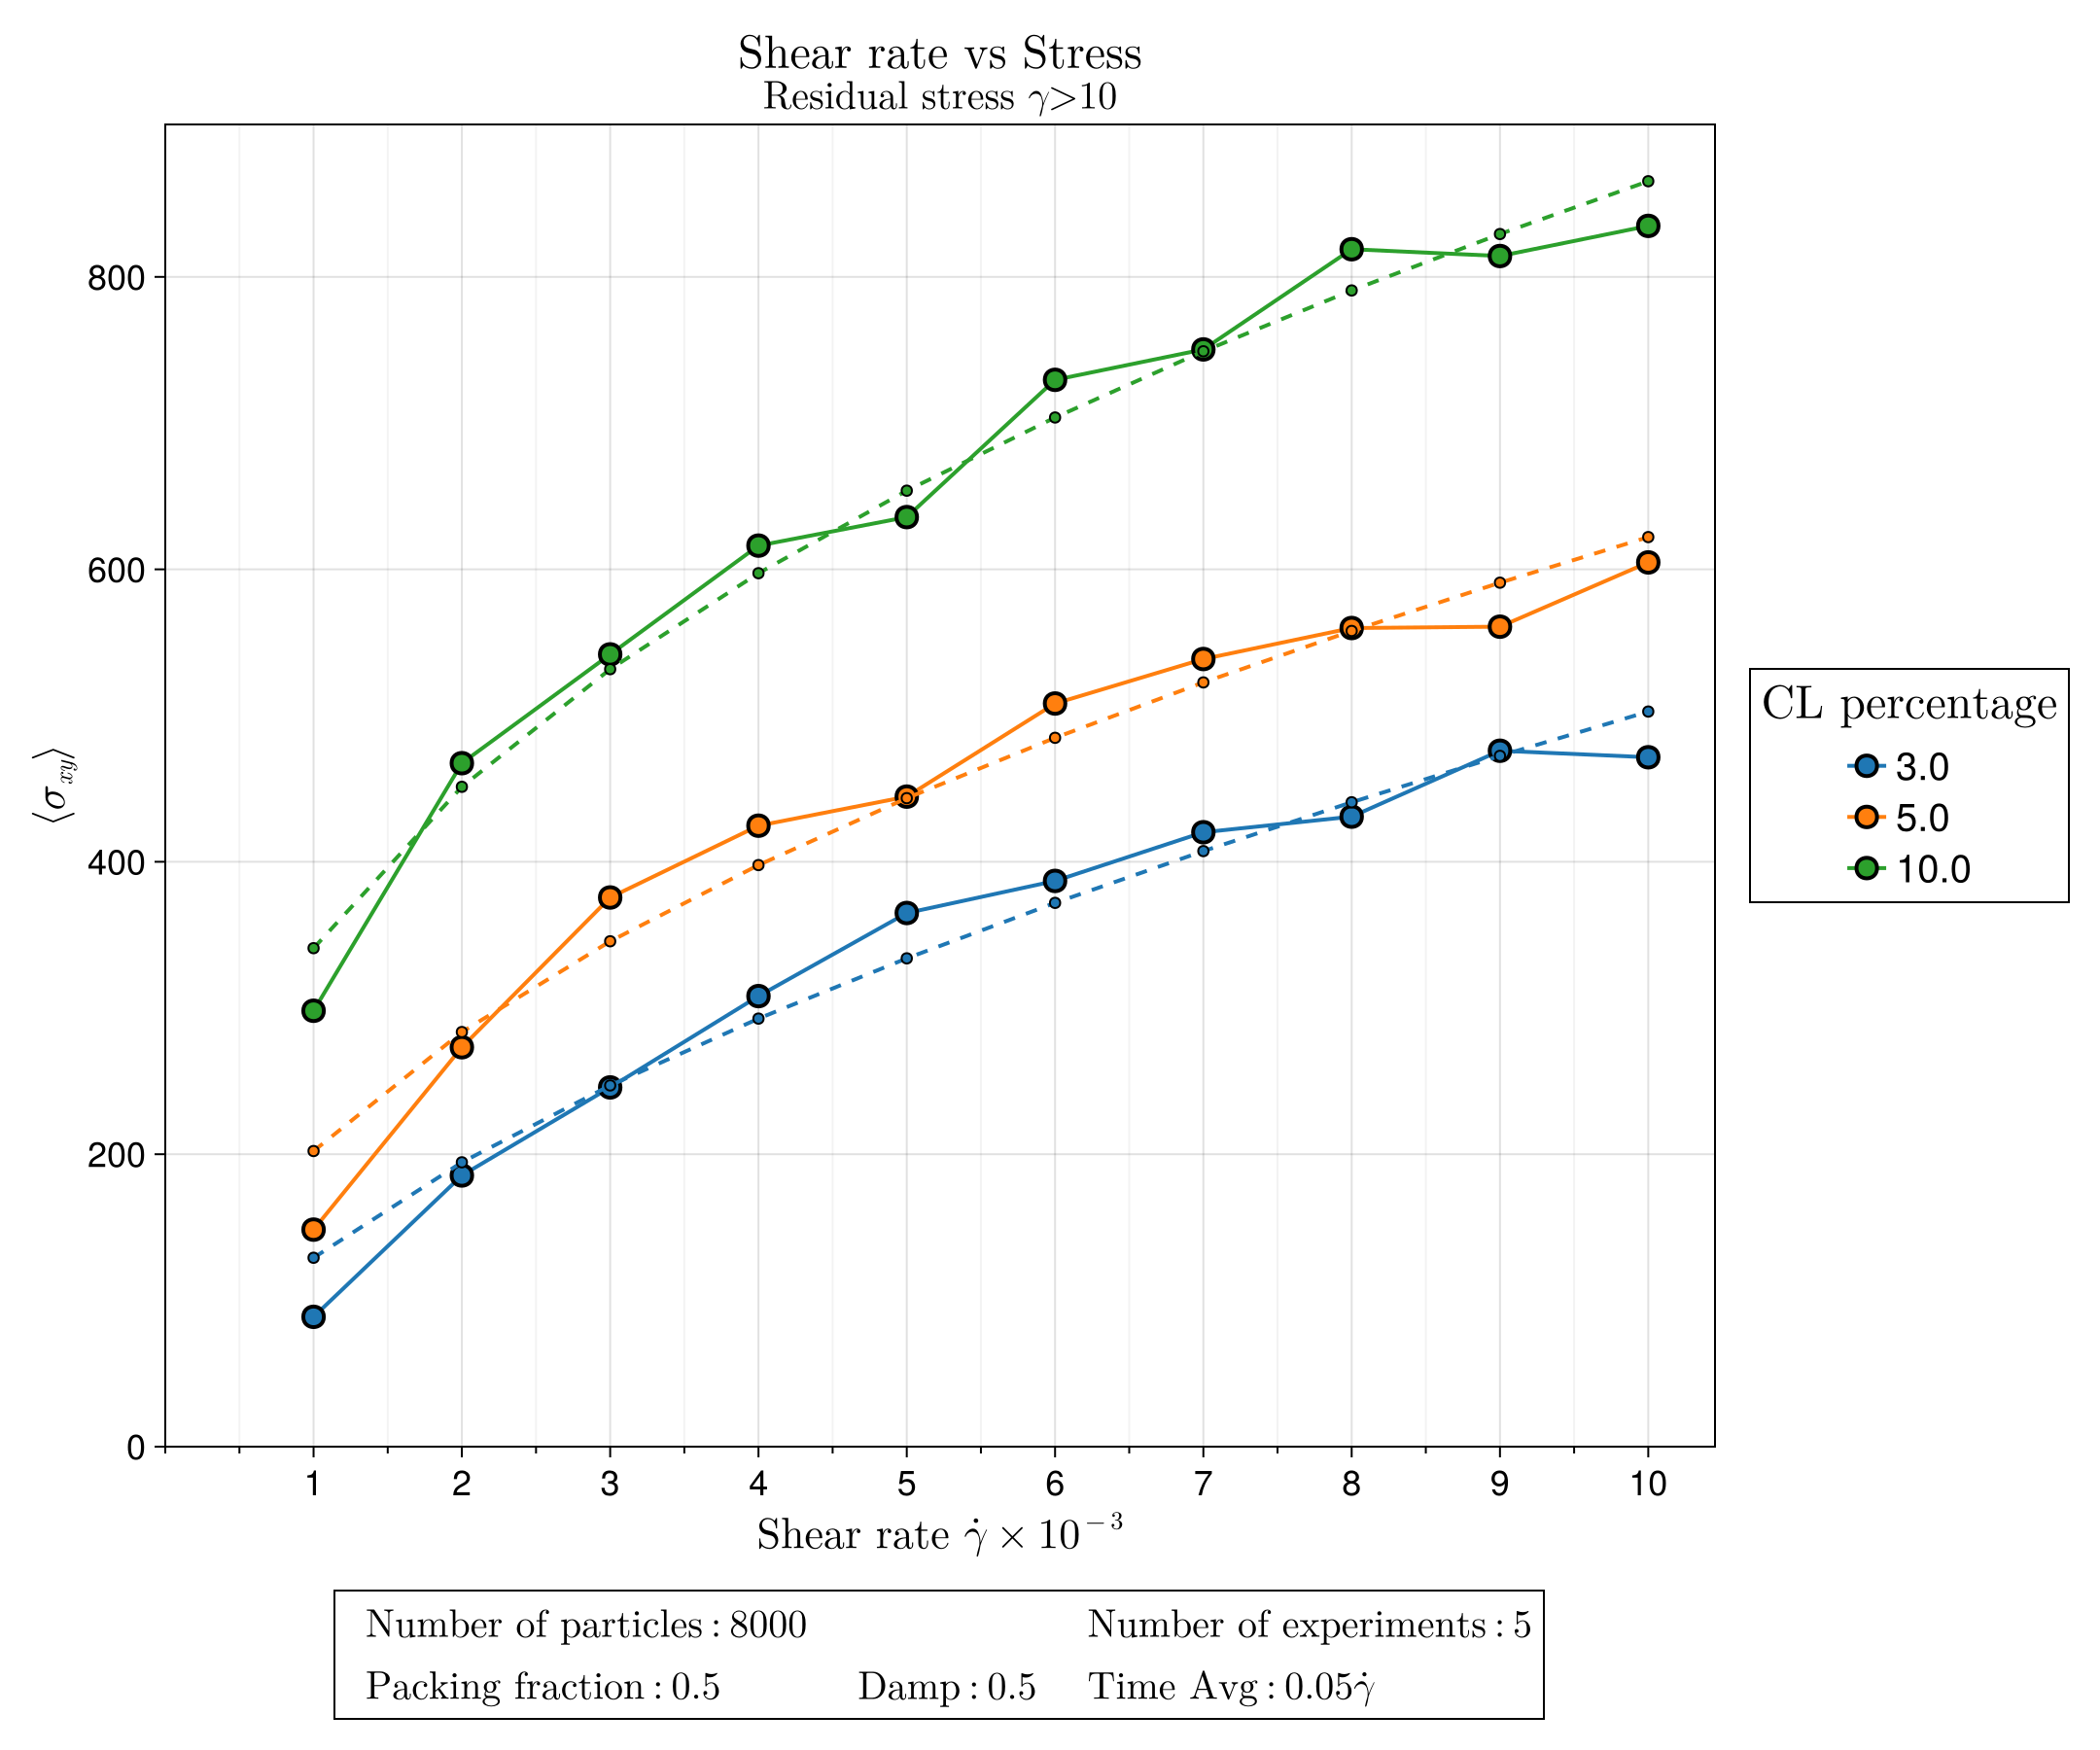
\includegraphics[width=\textwidth]{figs/ComputaitonalResults/yieldStress.png}
    \caption{Yield stress from computational results}\label{fig:yieldStressResults}
\end{figure}

\begin{gather}
    m(p_1,p_2,\dot{\gamma}) = p_1\dot{\gamma}^{p_2}.
\end{gather}

$p_2 = \{0.5901,0.4880,0.4045\}$

\subsection{Network analysis}

I guess that figures of the final network and parameter of order or size of porous or whatever.

